\documentclass[11pt]{article}
\usepackage[margin=2cm]{geometry}
\usepackage{amsmath,amssymb}
\usepackage{graphicx}
\usepackage{booktabs}
\usepackage{array}
\usepackage{xcolor}
\usepackage[breakable]{tcolorbox}
\usepackage{enumitem}
\usepackage[hidelinks]{hyperref}
\allowdisplaybreaks
\setlength{\parindent}{0pt}
\setlength{\parskip}{4pt}
\definecolor{stepc}{HTML}{1F4E9E}
\definecolor{ansc}{HTML}{0B6E4F}
\newcommand{\solstep}[2]{\par\medskip{\color{stepc}\textbf{Step #1 --- #2}}\par\nopagebreak}
\newtcolorbox{probbox}[1]{colback=white,colframe=black!55,fonttitle=\bfseries,title={#1}}
\newtcolorbox{ansbox}{breakable,colback=ansc!6,colframe=ansc,fonttitle=\bfseries,title={Answer}}
\newtcolorbox{cardbox}[1]{breakable,colback=stepc!4,colframe=stepc,fonttitle=\bfseries,title={#1}}
\graphicspath{{../../../output/lecture4/4B_current_mirrors/}}
\title{Set 4B: BJT Biasing with Current Mirrors}
\author{ECEN 325 --- Lecture 4 (Bipolar Junction Transistors) practice set}
\date{}
\begin{document}
\maketitle

\textbf{What this set trains.} DC analysis when the bias currents come from current mirrors. The reference current is
set by a resistor and diode-connected transistor(s); every transistor that shares the base and emitter nodes of a
diode-connected transistor copies its current. Then continue node by node as in set 4A and verify the assumptions.
$\beta = 100$ throughout. Problems 1--6 are easy, 7--12 medium, 13--18 hard. Try each problem before looking at its
solution.


\begin{cardbox}{The Lecture-4 pipeline (use it for every problem in this lecture)}
\textbf{Tools --- this is all the theory you need (plus the Lecture-1--3 tools):}
\begin{enumerate}[label=\textbf{T\arabic*},leftmargin=2.2em,itemsep=1pt]
\item \emph{Active BJT at DC:} npn $V_{BE}=0.7$\,V, pnp $V_{EB}=0.7$\,V; $I_C=\beta I_B$, $I_E=(\beta+1)I_B$, so
      $I_C\approx I_E$ and, when $\beta$ is large, $I_B\approx 0$. Active needs $|V_{CE}|\ge 0.2$\,V.
\item \emph{Current mirror:} transistors with the same base node and the same emitter node have the same $V_{BE}$,
      hence the same $I_C$.
\item \emph{Small-signal parameters:} $r_e = \frac{V_T}{I_C}$ ($V_T=25$\,mV), $\alpha=\frac{\beta}{\beta+1}$, $r_o=\infty$.
      For AC, DC supplies are ground and ``$\infty$'' capacitors are shorts.
\item \emph{Node impedances and gains:} $Z_{base}=(\beta+1)(r_e+Z_E)$, $Z_{emitter}=r_e+\frac{Z_B}{\beta+1}$,
      $Z_{collector}=\infty$;\ \ CE $\frac{v_c}{v_b}=-\alpha\frac{Z_C}{r_e+Z_E}$, CB $\frac{v_c}{v_e}=\alpha\frac{Z_C}{Z_{emitter}}$,
      CC $\frac{v_e}{v_b}=\frac{Z_E}{r_e+Z_E}$. $Z_C$, $Z_E$, $Z_B$ are everything else hanging on that node
      (including the input resistance of the next stage).
\end{enumerate}
\textbf{Steps:}
\begin{enumerate}[leftmargin=2.2em,itemsep=1pt]
\item \emph{DC:} assume every transistor active and $I_B\approx0$; walk through the circuit node by node
      (dividers, $V_{BE}$, KCL for $I_E$, $I_C\approx I_E$, collector voltages); then \emph{verify}: $I_B\ll$ bias currents and
      $|V_{CE}|\ge0.2$\,V.
\item \emph{AC:} $r_e$ of every transistor; input resistance of every stage from the last one backwards; multiply the
      node-to-node gains along the signal path; then standard form, Bode plot and output as in Lecture 1.
\item \emph{Design:} run the same relations backwards, choosing the free quantities with the stated design rules, then
      check the result by analysing the finished circuit.
\end{enumerate}
\end{cardbox}

\section*{Problems}
\subsection*{Easy problems}
\begin{probbox}{Problem 4B.1 \hfill Easy}
For the circuit below, find the DC collector currents $I_C$ of all transistors and verify all assumptions, including the operating region of every transistor. Assume $\beta = 100$.
\begin{center}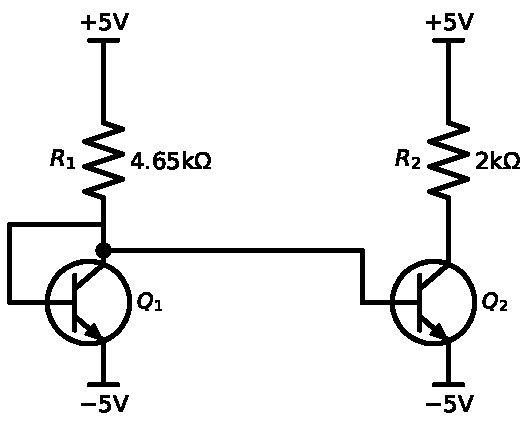
\includegraphics[width=\linewidth,height=7cm,keepaspectratio]{p01_circuit}\end{center}
\end{probbox}

\begin{probbox}{Problem 4B.2 \hfill Easy}
For the circuit below, find the DC collector currents $I_C$ of all transistors and verify all assumptions, including the operating region of every transistor. Assume $\beta = 100$.
\begin{center}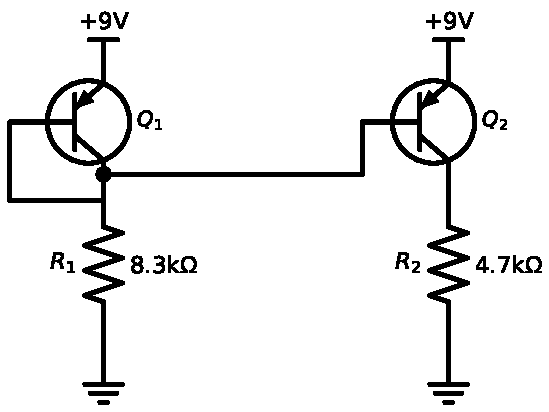
\includegraphics[width=\linewidth,height=7cm,keepaspectratio]{p02_circuit}\end{center}
\end{probbox}

\begin{probbox}{Problem 4B.3 \hfill Easy}
For the circuit below, find the DC collector currents $I_C$ of all transistors and verify all assumptions, including the operating region of every transistor. Assume $\beta = 100$.
\begin{center}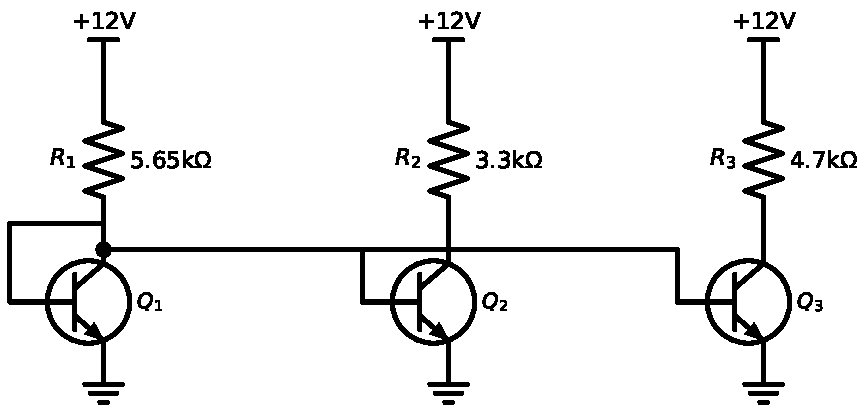
\includegraphics[width=\linewidth,height=7cm,keepaspectratio]{p03_circuit}\end{center}
\end{probbox}

\begin{probbox}{Problem 4B.4 \hfill Easy}
For the circuit below, find the DC collector currents $I_C$ of all transistors and verify all assumptions, including the operating region of every transistor. Assume $\beta = 100$.
\begin{center}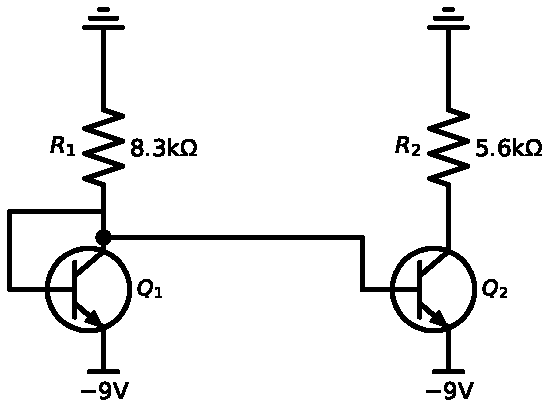
\includegraphics[width=\linewidth,height=7cm,keepaspectratio]{p04_circuit}\end{center}
\end{probbox}

\begin{probbox}{Problem 4B.5 \hfill Easy}
For the circuit below, find the DC collector currents $I_C$ of all transistors and verify all assumptions, including the operating region of every transistor. Assume $\beta = 100$.
\begin{center}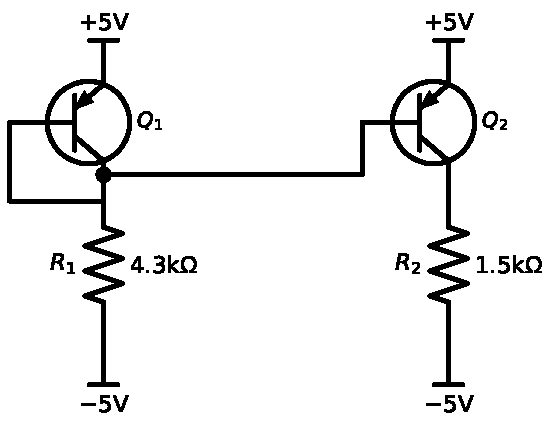
\includegraphics[width=\linewidth,height=7cm,keepaspectratio]{p05_circuit}\end{center}
\end{probbox}

\begin{probbox}{Problem 4B.6 \hfill Easy}
For the circuit below, find the DC collector currents $I_C$ of all transistors and verify all assumptions, including the operating region of every transistor. Assume $\beta = 100$.
\begin{center}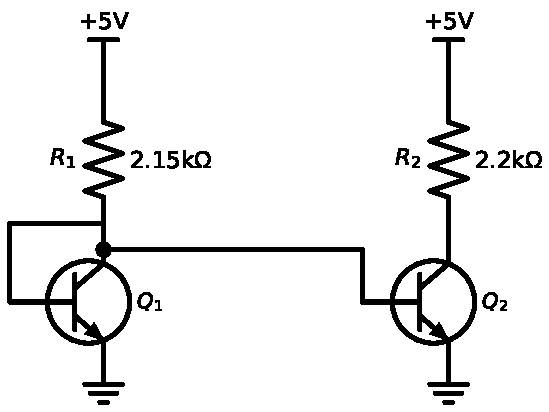
\includegraphics[width=\linewidth,height=7cm,keepaspectratio]{p06_circuit}\end{center}
\end{probbox}

\subsection*{Medium problems}
\begin{probbox}{Problem 4B.7 \hfill Medium}
For the circuit below, find the DC collector currents $I_C$ of all transistors and verify all assumptions, including the operating region of every transistor. Assume $\beta = 100$.
\begin{center}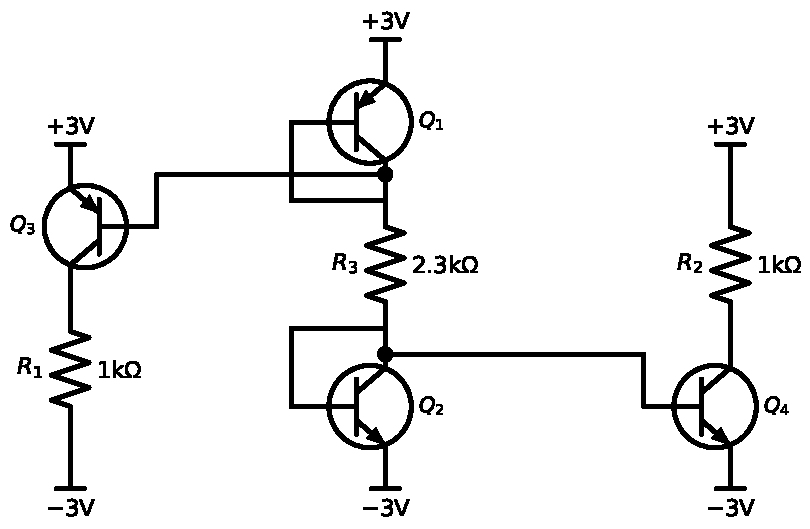
\includegraphics[width=\linewidth,height=7cm,keepaspectratio]{p07_circuit}\end{center}
\end{probbox}

\begin{probbox}{Problem 4B.8 \hfill Medium}
For the circuit below, find the DC collector currents $I_C$ of all transistors and verify all assumptions, including the operating region of every transistor. Assume $\beta = 100$.
\begin{center}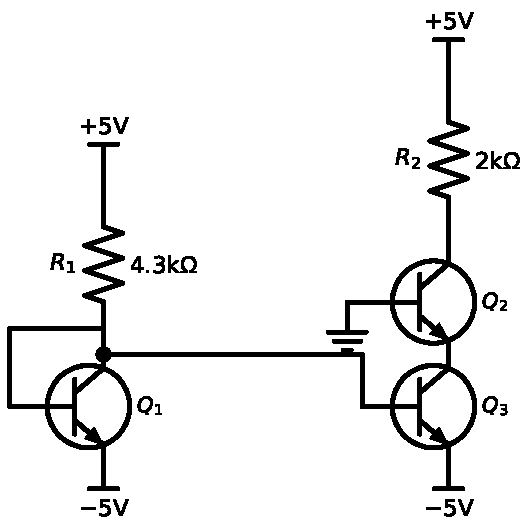
\includegraphics[width=\linewidth,height=7cm,keepaspectratio]{p08_circuit}\end{center}
\end{probbox}

\begin{probbox}{Problem 4B.9 \hfill Medium}
For the circuit below, find the DC collector currents $I_C$ of all transistors and verify all assumptions, including the operating region of every transistor. Assume $\beta = 100$.
\begin{center}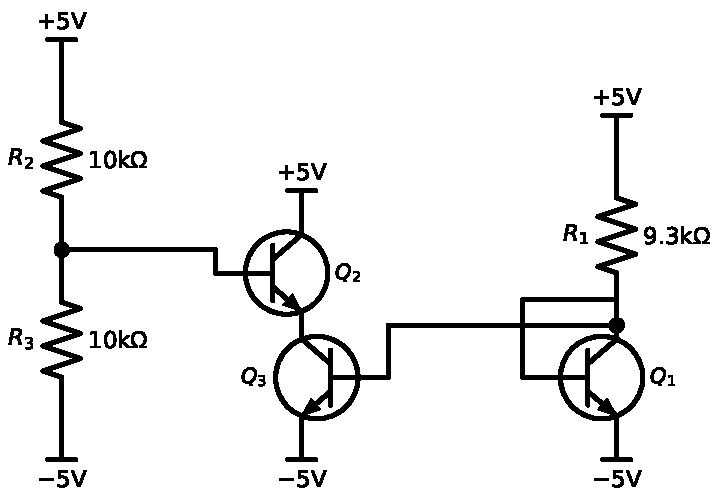
\includegraphics[width=\linewidth,height=7cm,keepaspectratio]{p09_circuit}\end{center}
\end{probbox}

\begin{probbox}{Problem 4B.10 \hfill Medium}
For the circuit below, find the DC collector currents $I_C$ of all transistors and verify all assumptions, including the operating region of every transistor. Assume $\beta = 100$.
\begin{center}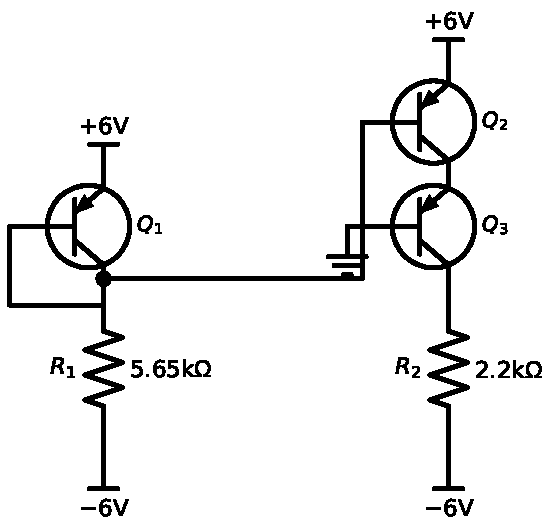
\includegraphics[width=\linewidth,height=7cm,keepaspectratio]{p10_circuit}\end{center}
\end{probbox}

\begin{probbox}{Problem 4B.11 \hfill Medium}
For the circuit below, find the DC collector currents $I_C$ of all transistors and verify all assumptions, including the operating region of every transistor. Assume $\beta = 100$.
\begin{center}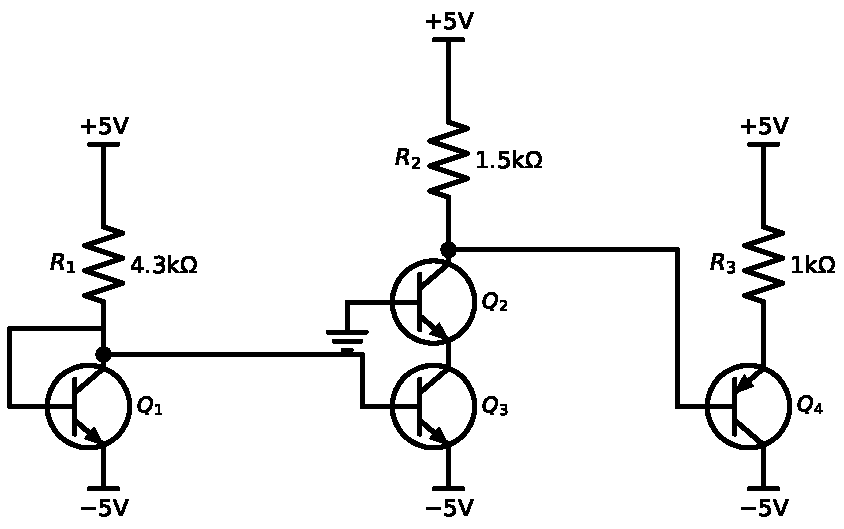
\includegraphics[width=\linewidth,height=7cm,keepaspectratio]{p11_circuit}\end{center}
\end{probbox}

\begin{probbox}{Problem 4B.12 \hfill Medium}
For the circuit below, find the DC collector currents $I_C$ of all transistors and verify all assumptions, including the operating region of every transistor. Assume $\beta = 100$.
\begin{center}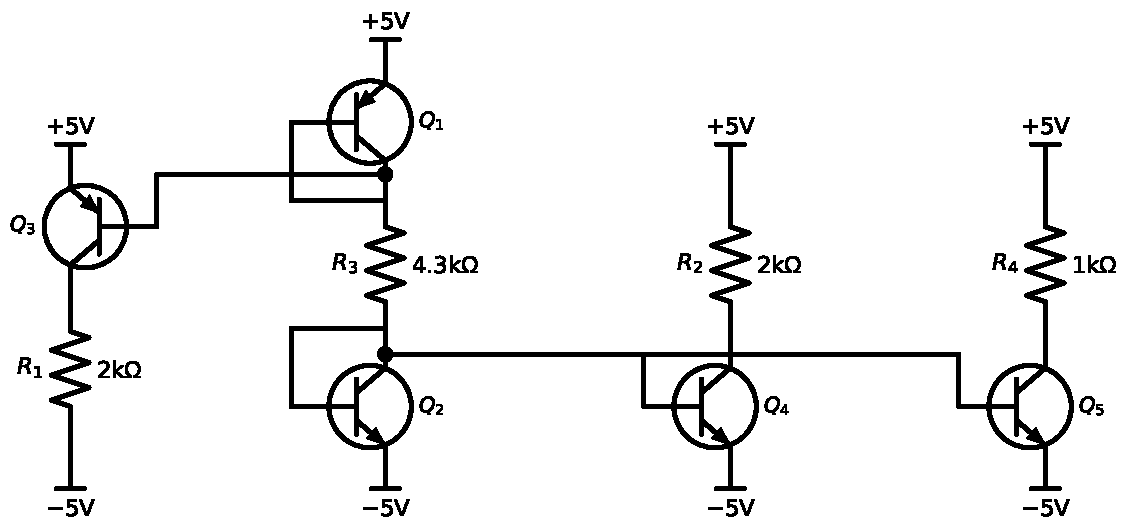
\includegraphics[width=\linewidth,height=7cm,keepaspectratio]{p12_circuit}\end{center}
\end{probbox}

\subsection*{Hard problems}
\begin{probbox}{Problem 4B.13 \hfill Hard}
For the circuit below, find the DC collector currents $I_C$ of all transistors and verify all assumptions, including the operating region of every transistor. Assume $\beta = 100$.
\begin{center}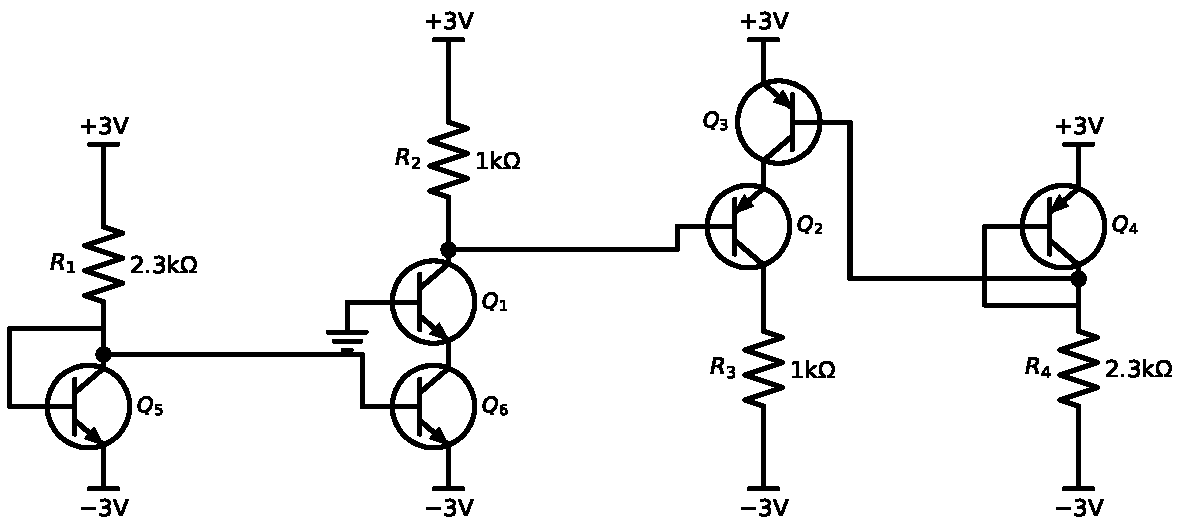
\includegraphics[width=\linewidth,height=7cm,keepaspectratio]{p13_circuit}\end{center}
\end{probbox}

\begin{probbox}{Problem 4B.14 \hfill Hard}
For the circuit below, find the DC collector currents $I_C$ of all transistors and verify all assumptions, including the operating region of every transistor. Assume $\beta = 100$.
\begin{center}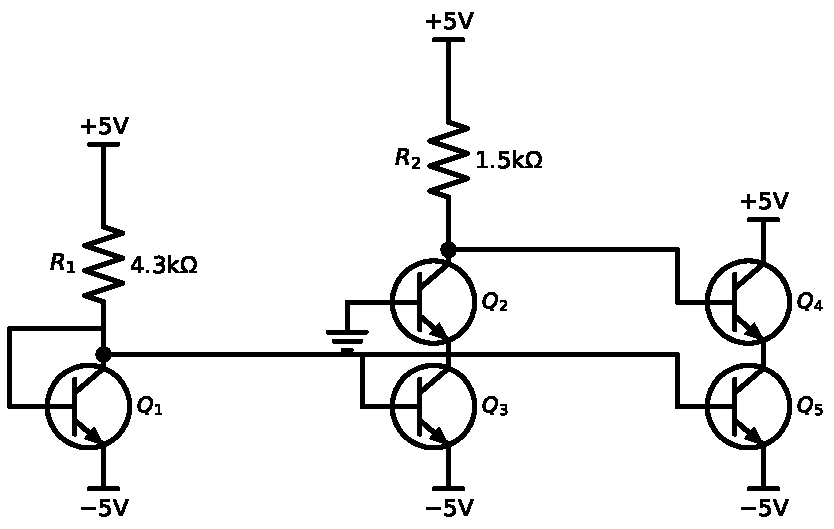
\includegraphics[width=\linewidth,height=7cm,keepaspectratio]{p14_circuit}\end{center}
\end{probbox}

\begin{probbox}{Problem 4B.15 \hfill Hard}
For the circuit below, find the DC collector currents $I_C$ of all transistors and verify all assumptions, including the operating region of every transistor. Assume $\beta = 100$.
\begin{center}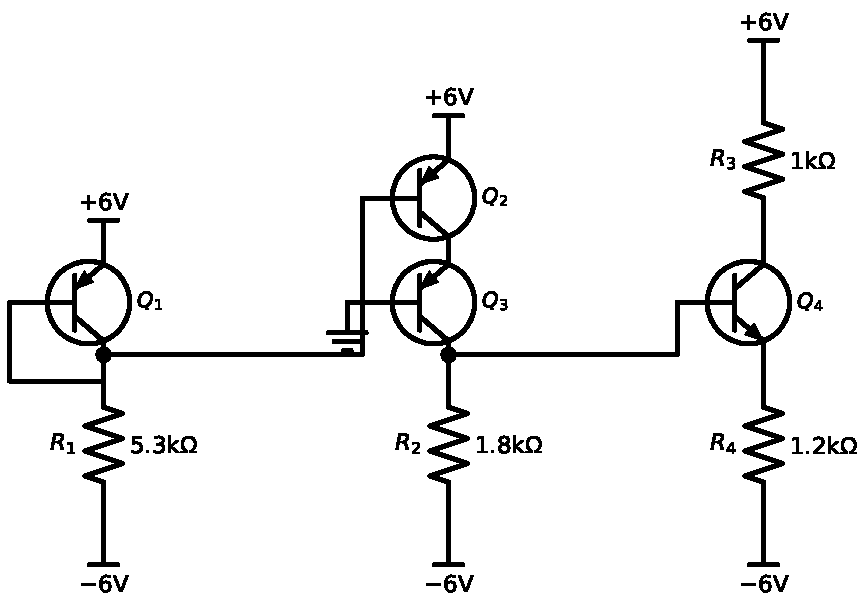
\includegraphics[width=\linewidth,height=7cm,keepaspectratio]{p15_circuit}\end{center}
\end{probbox}

\begin{probbox}{Problem 4B.16 \hfill Hard}
For the circuit below, find the DC collector currents $I_C$ of all transistors and verify all assumptions, including the operating region of every transistor. Assume $\beta = 100$.
\begin{center}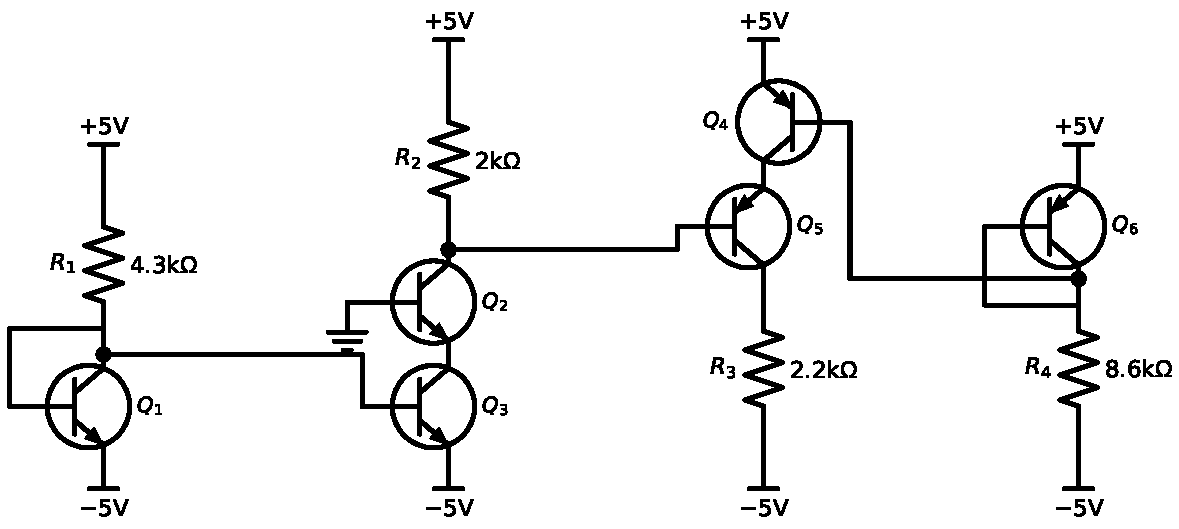
\includegraphics[width=\linewidth,height=7cm,keepaspectratio]{p16_circuit}\end{center}
\end{probbox}

\begin{probbox}{Problem 4B.17 \hfill Hard}
For the circuit below, find the DC collector currents $I_C$ of all transistors and verify all assumptions, including the operating region of every transistor. Assume $\beta = 100$.
\begin{center}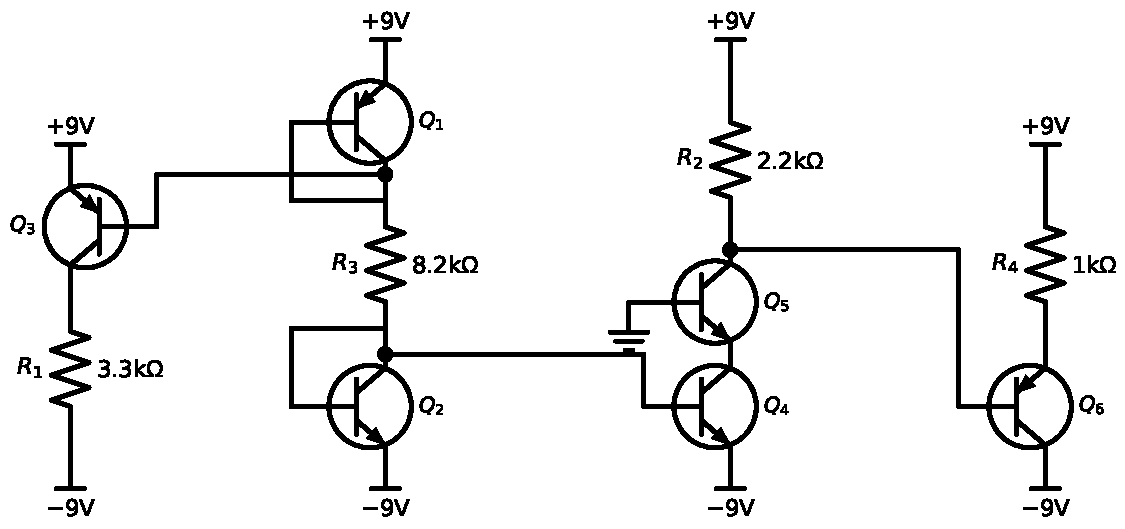
\includegraphics[width=\linewidth,height=7cm,keepaspectratio]{p17_circuit}\end{center}
\end{probbox}

\begin{probbox}{Problem 4B.18 \hfill Hard}
For the circuit below, find the DC collector currents $I_C$ of all transistors and verify all assumptions, including the operating region of every transistor. Assume $\beta = 100$.
\begin{center}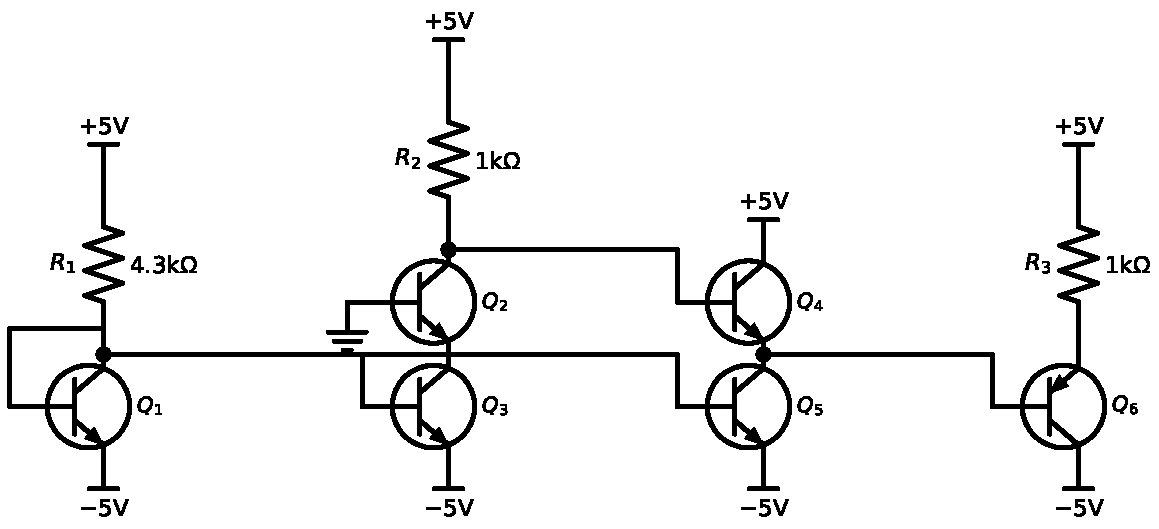
\includegraphics[width=\linewidth,height=7cm,keepaspectratio]{p18_circuit}\end{center}
\end{probbox}

\newpage
\section*{Solutions}
Every solution follows the steps of the Lecture-4 pipeline card.
\subsection*{Solution 4B.1 \hfill Easy}
\begin{center}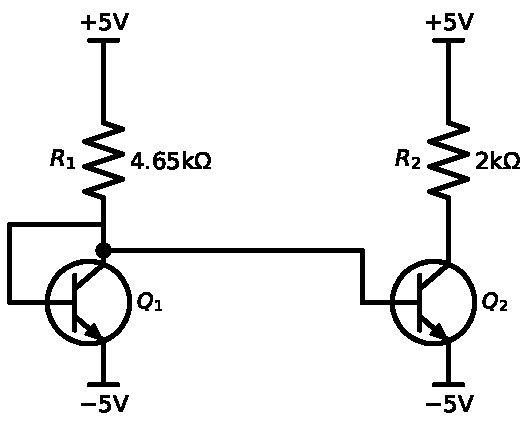
\includegraphics[width=0.9\linewidth,height=6cm,keepaspectratio]{p01_circuit}\end{center}
\solstep{1}{Assumptions}Assume every transistor is in the active region and that every base current is negligible ($I_B\approx0$, tool T1): then $|V_{BE}| = 0.7$\,V, $I_C\approx I_E$, and no current flows into any base, so a base network behaves like a plain resistor divider.
\solstep{2}{Walk through the circuit}\begin{enumerate}[leftmargin=*,itemsep=3pt]
\item $Q_{1}$ (diode-connected) is active: $V_{B1} = (-5) + 0.7 = -4.3\,\mathrm{V}$.
\item KCL at the collector of $Q_{1}$ (base current neglected): \[I_{C1} = \frac{5 - V_{B1}}{R_{1}} = 2\,\mathrm{m}\mathrm{A}\]
\item $Q_{2}$ has the same base and emitter nodes as $Q_{1}$, hence the same $V_{BE}$ and the same current (current mirror): $I_{C2} = I_{C1} = 2\,\mathrm{m}\mathrm{A}$.
\item $Q_{2}$ draws $I_{C2} = 2\,\mathrm{m}\mathrm{A}$ from $V_{C2}$ through $R_{2}$: $V_{C2} = 5 - R_{2}\,(I_{C2}) = 5 - 2\,\mathrm{k}\times2\,\mathrm{m}\mathrm{A} = 1\,\mathrm{V}$.
\end{enumerate}

\solstep{3}{Verify the assumptions}\begin{itemize}[leftmargin=*,itemsep=2pt]
\item $I_{B1} = \frac{I_{C1}}{\beta} = 20\,\mu \mathrm{A}$ (all bases on this node: $40\,\mu \mathrm{A}$) $\ll$ the $2\,\mathrm{m}\mathrm{A}$ flowing in the base network \checkmark
\item $I_{B2} = \frac{I_{C2}}{\beta} = 20\,\mu \mathrm{A}$ (all bases on this node: $40\,\mu \mathrm{A}$) $\ll$ the $2\,\mathrm{m}\mathrm{A}$ flowing in the base network \checkmark
\item $V_{CE1} = V_{B1} - (-5) = -4.3 - (-5) = 0.7\,\mathrm{V}$ $\ge 0.2$\,V $\Rightarrow$ $Q_{1}$ is active \checkmark
\item $V_{CE2} = V_{C2} - (-5) = 1 - (-5) = 6\,\mathrm{V}$ $\ge 0.2$\,V $\Rightarrow$ $Q_{2}$ is active \checkmark
\end{itemize}

\solstep{4}{How good was $I_B\approx 0$?}If we keep the base currents ($I_C=\beta I_B$ with $\beta=100$) and solve the circuit exactly, the currents change only a little:\begin{center}\renewcommand{\arraystretch}{1.35}
\begin{tabular}{cccc}
\toprule
transistor & $I_C$ (with $I_B\approx0$) & $I_C$ (exact) & difference \\
\midrule
$Q_{1}$ & $2\,\mathrm{m}\mathrm{A}$ & $1.96\,\mathrm{m}\mathrm{A}$ & $2\%$ \\
$Q_{2}$ & $2\,\mathrm{m}\mathrm{A}$ & $1.96\,\mathrm{m}\mathrm{A}$ & $2\%$ \\
\bottomrule
\end{tabular}\end{center}

\begin{ansbox}
$I_{C1} = 2\,\mathrm{m}\mathrm{A}$,\quad $I_{C2} = 2\,\mathrm{m}\mathrm{A}$\\[2pt] all transistors active, all base currents negligible.
\end{ansbox}

\newpage
\subsection*{Solution 4B.2 \hfill Easy}
\begin{center}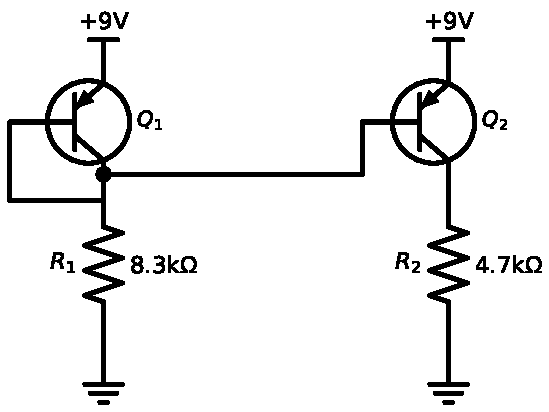
\includegraphics[width=0.9\linewidth,height=6cm,keepaspectratio]{p02_circuit}\end{center}
\solstep{1}{Assumptions}Assume every transistor is in the active region and that every base current is negligible ($I_B\approx0$, tool T1): then $|V_{BE}| = 0.7$\,V, $I_C\approx I_E$, and no current flows into any base, so a base network behaves like a plain resistor divider.
\solstep{2}{Walk through the circuit}\begin{enumerate}[leftmargin=*,itemsep=3pt]
\item $Q_{1}$ (diode-connected) is active: $V_{B1} = 9 - 0.7 = 8.3\,\mathrm{V}$.
\item KCL at the collector of $Q_{1}$ (base current neglected): \[I_{C1} = \frac{V_{B1} - 0}{R_{1}} = 1\,\mathrm{m}\mathrm{A}\]
\item $Q_{2}$ has the same base and emitter nodes as $Q_{1}$, hence the same $V_{BE}$ and the same current (current mirror): $I_{C2} = I_{C1} = 1\,\mathrm{m}\mathrm{A}$.
\item The current $I_{C2} = 1\,\mathrm{m}\mathrm{A}$ flows from $V_{C2}$ through $R_{2}$: $V_{C2} = 0 + R_{2}\,(I_{C2}) = 0 + 4.7\,\mathrm{k}\times1\,\mathrm{m}\mathrm{A} = 4.7\,\mathrm{V}$.
\end{enumerate}

\solstep{3}{Verify the assumptions}\begin{itemize}[leftmargin=*,itemsep=2pt]
\item $I_{B1} = \frac{I_{C1}}{\beta} = 10\,\mu \mathrm{A}$ (all bases on this node: $20\,\mu \mathrm{A}$) $\ll$ the $1\,\mathrm{m}\mathrm{A}$ flowing in the base network \checkmark
\item $I_{B2} = \frac{I_{C2}}{\beta} = 10\,\mu \mathrm{A}$ (all bases on this node: $20\,\mu \mathrm{A}$) $\ll$ the $1\,\mathrm{m}\mathrm{A}$ flowing in the base network \checkmark
\item $V_{EC1} = 9 - V_{B1} = 9 - (8.3) = 0.7\,\mathrm{V}$ $\ge 0.2$\,V $\Rightarrow$ $Q_{1}$ is active \checkmark
\item $V_{EC2} = 9 - V_{C2} = 9 - (4.7) = 4.3\,\mathrm{V}$ $\ge 0.2$\,V $\Rightarrow$ $Q_{2}$ is active \checkmark
\end{itemize}

\solstep{4}{How good was $I_B\approx 0$?}If we keep the base currents ($I_C=\beta I_B$ with $\beta=100$) and solve the circuit exactly, the currents change only a little:\begin{center}\renewcommand{\arraystretch}{1.35}
\begin{tabular}{cccc}
\toprule
transistor & $I_C$ (with $I_B\approx0$) & $I_C$ (exact) & difference \\
\midrule
$Q_{1}$ & $1\,\mathrm{m}\mathrm{A}$ & $980\,\mu \mathrm{A}$ & $2\%$ \\
$Q_{2}$ & $1\,\mathrm{m}\mathrm{A}$ & $980\,\mu \mathrm{A}$ & $2\%$ \\
\bottomrule
\end{tabular}\end{center}

\begin{ansbox}
$I_{C1} = 1\,\mathrm{m}\mathrm{A}$,\quad $I_{C2} = 1\,\mathrm{m}\mathrm{A}$\\[2pt] all transistors active, all base currents negligible.
\end{ansbox}

\newpage
\subsection*{Solution 4B.3 \hfill Easy}
\begin{center}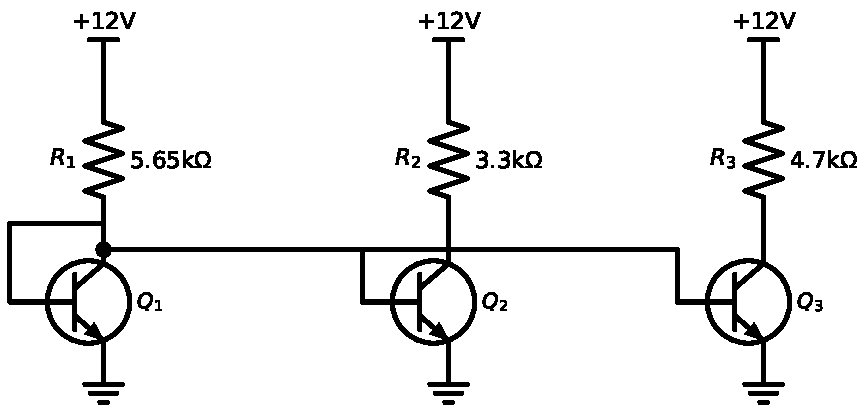
\includegraphics[width=0.9\linewidth,height=6cm,keepaspectratio]{p03_circuit}\end{center}
\solstep{1}{Assumptions}Assume every transistor is in the active region and that every base current is negligible ($I_B\approx0$, tool T1): then $|V_{BE}| = 0.7$\,V, $I_C\approx I_E$, and no current flows into any base, so a base network behaves like a plain resistor divider.
\solstep{2}{Walk through the circuit}\begin{enumerate}[leftmargin=*,itemsep=3pt]
\item $Q_{1}$ (diode-connected) is active: $V_{B1} = 0 + 0.7 = 0.7\,\mathrm{V}$.
\item KCL at the collector of $Q_{1}$ (base current neglected): \[I_{C1} = \frac{12 - V_{B1}}{R_{1}} = 2\,\mathrm{m}\mathrm{A}\]
\item $Q_{2}$ has the same base and emitter nodes as $Q_{1}$, hence the same $V_{BE}$ and the same current (current mirror): $I_{C2} = I_{C1} = 2\,\mathrm{m}\mathrm{A}$.
\item $Q_{3}$ has the same base and emitter nodes as $Q_{1}$, hence the same $V_{BE}$ and the same current (current mirror): $I_{C3} = I_{C1} = 2\,\mathrm{m}\mathrm{A}$.
\item $Q_{2}$ draws $I_{C2} = 2\,\mathrm{m}\mathrm{A}$ from $V_{C2}$ through $R_{2}$: $V_{C2} = 12 - R_{2}\,(I_{C2}) = 12 - 3.3\,\mathrm{k}\times2\,\mathrm{m}\mathrm{A} = 5.4\,\mathrm{V}$.
\item $Q_{3}$ draws $I_{C3} = 2\,\mathrm{m}\mathrm{A}$ from $V_{C3}$ through $R_{3}$: $V_{C3} = 12 - R_{3}\,(I_{C3}) = 12 - 4.7\,\mathrm{k}\times2\,\mathrm{m}\mathrm{A} = 2.6\,\mathrm{V}$.
\end{enumerate}

\solstep{3}{Verify the assumptions}\begin{itemize}[leftmargin=*,itemsep=2pt]
\item $I_{B1} = \frac{I_{C1}}{\beta} = 20\,\mu \mathrm{A}$ (all bases on this node: $60\,\mu \mathrm{A}$) $\ll$ the $2\,\mathrm{m}\mathrm{A}$ flowing in the base network \checkmark
\item $I_{B2} = \frac{I_{C2}}{\beta} = 20\,\mu \mathrm{A}$ (all bases on this node: $60\,\mu \mathrm{A}$) $\ll$ the $2\,\mathrm{m}\mathrm{A}$ flowing in the base network \checkmark
\item $I_{B3} = \frac{I_{C3}}{\beta} = 20\,\mu \mathrm{A}$ (all bases on this node: $60\,\mu \mathrm{A}$) $\ll$ the $2\,\mathrm{m}\mathrm{A}$ flowing in the base network \checkmark
\item $V_{CE1} = V_{B1} - 0 = 0.7 - (0) = 0.7\,\mathrm{V}$ $\ge 0.2$\,V $\Rightarrow$ $Q_{1}$ is active \checkmark
\item $V_{CE2} = V_{C2} - 0 = 5.4 - (0) = 5.4\,\mathrm{V}$ $\ge 0.2$\,V $\Rightarrow$ $Q_{2}$ is active \checkmark
\item $V_{CE3} = V_{C3} - 0 = 2.6 - (0) = 2.6\,\mathrm{V}$ $\ge 0.2$\,V $\Rightarrow$ $Q_{3}$ is active \checkmark
\end{itemize}

\solstep{4}{How good was $I_B\approx 0$?}If we keep the base currents ($I_C=\beta I_B$ with $\beta=100$) and solve the circuit exactly, the currents change only a little:\begin{center}\renewcommand{\arraystretch}{1.35}
\begin{tabular}{cccc}
\toprule
transistor & $I_C$ (with $I_B\approx0$) & $I_C$ (exact) & difference \\
\midrule
$Q_{1}$ & $2\,\mathrm{m}\mathrm{A}$ & $1.94\,\mathrm{m}\mathrm{A}$ & $3\%$ \\
$Q_{2}$ & $2\,\mathrm{m}\mathrm{A}$ & $1.94\,\mathrm{m}\mathrm{A}$ & $3\%$ \\
$Q_{3}$ & $2\,\mathrm{m}\mathrm{A}$ & $1.94\,\mathrm{m}\mathrm{A}$ & $3\%$ \\
\bottomrule
\end{tabular}\end{center}

\begin{ansbox}
$I_{C1} = 2\,\mathrm{m}\mathrm{A}$,\quad $I_{C2} = 2\,\mathrm{m}\mathrm{A}$,\quad $I_{C3} = 2\,\mathrm{m}\mathrm{A}$\\[2pt] all transistors active, all base currents negligible.
\end{ansbox}

\newpage
\subsection*{Solution 4B.4 \hfill Easy}
\begin{center}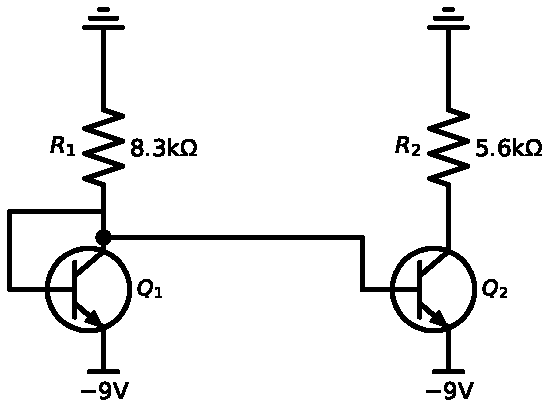
\includegraphics[width=0.9\linewidth,height=6cm,keepaspectratio]{p04_circuit}\end{center}
\solstep{1}{Assumptions}Assume every transistor is in the active region and that every base current is negligible ($I_B\approx0$, tool T1): then $|V_{BE}| = 0.7$\,V, $I_C\approx I_E$, and no current flows into any base, so a base network behaves like a plain resistor divider.
\solstep{2}{Walk through the circuit}\begin{enumerate}[leftmargin=*,itemsep=3pt]
\item $Q_{1}$ (diode-connected) is active: $V_{B1} = (-9) + 0.7 = -8.3\,\mathrm{V}$.
\item KCL at the collector of $Q_{1}$ (base current neglected): \[I_{C1} = \frac{0 - V_{B1}}{R_{1}} = 1\,\mathrm{m}\mathrm{A}\]
\item $Q_{2}$ has the same base and emitter nodes as $Q_{1}$, hence the same $V_{BE}$ and the same current (current mirror): $I_{C2} = I_{C1} = 1\,\mathrm{m}\mathrm{A}$.
\item $Q_{2}$ draws $I_{C2} = 1\,\mathrm{m}\mathrm{A}$ from $V_{C2}$ through $R_{2}$: $V_{C2} = 0 - R_{2}\,(I_{C2}) = 0 - 5.6\,\mathrm{k}\times1\,\mathrm{m}\mathrm{A} = -5.6\,\mathrm{V}$.
\end{enumerate}

\solstep{3}{Verify the assumptions}\begin{itemize}[leftmargin=*,itemsep=2pt]
\item $I_{B1} = \frac{I_{C1}}{\beta} = 10\,\mu \mathrm{A}$ (all bases on this node: $20\,\mu \mathrm{A}$) $\ll$ the $1\,\mathrm{m}\mathrm{A}$ flowing in the base network \checkmark
\item $I_{B2} = \frac{I_{C2}}{\beta} = 10\,\mu \mathrm{A}$ (all bases on this node: $20\,\mu \mathrm{A}$) $\ll$ the $1\,\mathrm{m}\mathrm{A}$ flowing in the base network \checkmark
\item $V_{CE1} = V_{B1} - (-9) = -8.3 - (-9) = 0.7\,\mathrm{V}$ $\ge 0.2$\,V $\Rightarrow$ $Q_{1}$ is active \checkmark
\item $V_{CE2} = V_{C2} - (-9) = -5.6 - (-9) = 3.4\,\mathrm{V}$ $\ge 0.2$\,V $\Rightarrow$ $Q_{2}$ is active \checkmark
\end{itemize}

\solstep{4}{How good was $I_B\approx 0$?}If we keep the base currents ($I_C=\beta I_B$ with $\beta=100$) and solve the circuit exactly, the currents change only a little:\begin{center}\renewcommand{\arraystretch}{1.35}
\begin{tabular}{cccc}
\toprule
transistor & $I_C$ (with $I_B\approx0$) & $I_C$ (exact) & difference \\
\midrule
$Q_{1}$ & $1\,\mathrm{m}\mathrm{A}$ & $980\,\mu \mathrm{A}$ & $2\%$ \\
$Q_{2}$ & $1\,\mathrm{m}\mathrm{A}$ & $980\,\mu \mathrm{A}$ & $2\%$ \\
\bottomrule
\end{tabular}\end{center}

\begin{ansbox}
$I_{C1} = 1\,\mathrm{m}\mathrm{A}$,\quad $I_{C2} = 1\,\mathrm{m}\mathrm{A}$\\[2pt] all transistors active, all base currents negligible.
\end{ansbox}

\newpage
\subsection*{Solution 4B.5 \hfill Easy}
\begin{center}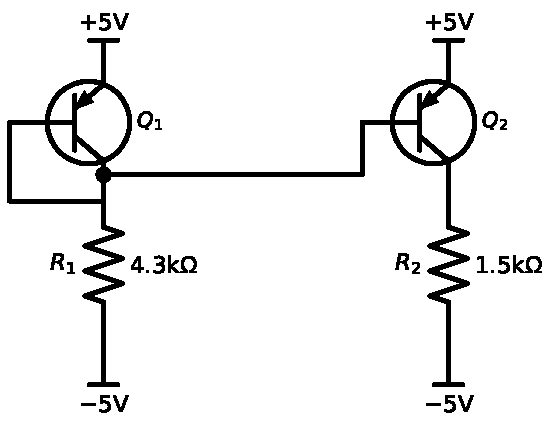
\includegraphics[width=0.9\linewidth,height=6cm,keepaspectratio]{p05_circuit}\end{center}
\solstep{1}{Assumptions}Assume every transistor is in the active region and that every base current is negligible ($I_B\approx0$, tool T1): then $|V_{BE}| = 0.7$\,V, $I_C\approx I_E$, and no current flows into any base, so a base network behaves like a plain resistor divider.
\solstep{2}{Walk through the circuit}\begin{enumerate}[leftmargin=*,itemsep=3pt]
\item $Q_{1}$ (diode-connected) is active: $V_{B1} = 5 - 0.7 = 4.3\,\mathrm{V}$.
\item KCL at the collector of $Q_{1}$ (base current neglected): \[I_{C1} = \frac{V_{B1} - (-5)}{R_{1}} = 2.16\,\mathrm{m}\mathrm{A}\]
\item $Q_{2}$ has the same base and emitter nodes as $Q_{1}$, hence the same $V_{BE}$ and the same current (current mirror): $I_{C2} = I_{C1} = 2.16\,\mathrm{m}\mathrm{A}$.
\item The current $I_{C2} = 2.16\,\mathrm{m}\mathrm{A}$ flows from $V_{C2}$ through $R_{2}$: $V_{C2} = (-5) + R_{2}\,(I_{C2}) = -5 + 1.5\,\mathrm{k}\times2.16\,\mathrm{m}\mathrm{A} = -1.76\,\mathrm{V}$.
\end{enumerate}

\solstep{3}{Verify the assumptions}\begin{itemize}[leftmargin=*,itemsep=2pt]
\item $I_{B1} = \frac{I_{C1}}{\beta} = 21.6\,\mu \mathrm{A}$ (all bases on this node: $43.3\,\mu \mathrm{A}$) $\ll$ the $2.16\,\mathrm{m}\mathrm{A}$ flowing in the base network \checkmark
\item $I_{B2} = \frac{I_{C2}}{\beta} = 21.6\,\mu \mathrm{A}$ (all bases on this node: $43.3\,\mu \mathrm{A}$) $\ll$ the $2.16\,\mathrm{m}\mathrm{A}$ flowing in the base network \checkmark
\item $V_{EC1} = 5 - V_{B1} = 5 - (4.3) = 0.7\,\mathrm{V}$ $\ge 0.2$\,V $\Rightarrow$ $Q_{1}$ is active \checkmark
\item $V_{EC2} = 5 - V_{C2} = 5 - (-1.756) = 6.76\,\mathrm{V}$ $\ge 0.2$\,V $\Rightarrow$ $Q_{2}$ is active \checkmark
\end{itemize}

\solstep{4}{How good was $I_B\approx 0$?}If we keep the base currents ($I_C=\beta I_B$ with $\beta=100$) and solve the circuit exactly, the currents change only a little:\begin{center}\renewcommand{\arraystretch}{1.35}
\begin{tabular}{cccc}
\toprule
transistor & $I_C$ (with $I_B\approx0$) & $I_C$ (exact) & difference \\
\midrule
$Q_{1}$ & $2.16\,\mathrm{m}\mathrm{A}$ & $2.12\,\mathrm{m}\mathrm{A}$ & $2\%$ \\
$Q_{2}$ & $2.16\,\mathrm{m}\mathrm{A}$ & $2.12\,\mathrm{m}\mathrm{A}$ & $2\%$ \\
\bottomrule
\end{tabular}\end{center}

\begin{ansbox}
$I_{C1} = 2.16\,\mathrm{m}\mathrm{A}$,\quad $I_{C2} = 2.16\,\mathrm{m}\mathrm{A}$\\[2pt] all transistors active, all base currents negligible.
\end{ansbox}

\newpage
\subsection*{Solution 4B.6 \hfill Easy}
\begin{center}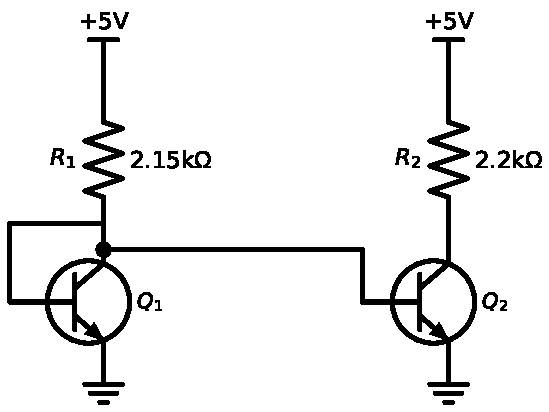
\includegraphics[width=0.9\linewidth,height=6cm,keepaspectratio]{p06_circuit}\end{center}
\solstep{1}{Assumptions}Assume every transistor is in the active region and that every base current is negligible ($I_B\approx0$, tool T1): then $|V_{BE}| = 0.7$\,V, $I_C\approx I_E$, and no current flows into any base, so a base network behaves like a plain resistor divider.
\solstep{2}{Walk through the circuit}\begin{enumerate}[leftmargin=*,itemsep=3pt]
\item $Q_{1}$ (diode-connected) is active: $V_{B1} = 0 + 0.7 = 0.7\,\mathrm{V}$.
\item KCL at the collector of $Q_{1}$ (base current neglected): \[I_{C1} = \frac{5 - V_{B1}}{R_{1}} = 2\,\mathrm{m}\mathrm{A}\]
\item $Q_{2}$ has the same base and emitter nodes as $Q_{1}$, hence the same $V_{BE}$ and the same current (current mirror): $I_{C2} = I_{C1} = 2\,\mathrm{m}\mathrm{A}$.
\item $Q_{2}$ draws $I_{C2} = 2\,\mathrm{m}\mathrm{A}$ from $V_{C2}$ through $R_{2}$: $V_{C2} = 5 - R_{2}\,(I_{C2}) = 5 - 2.2\,\mathrm{k}\times2\,\mathrm{m}\mathrm{A} = 0.6\,\mathrm{V}$.
\end{enumerate}

\solstep{3}{Verify the assumptions}\begin{itemize}[leftmargin=*,itemsep=2pt]
\item $I_{B1} = \frac{I_{C1}}{\beta} = 20\,\mu \mathrm{A}$ (all bases on this node: $40\,\mu \mathrm{A}$) $\ll$ the $2\,\mathrm{m}\mathrm{A}$ flowing in the base network \checkmark
\item $I_{B2} = \frac{I_{C2}}{\beta} = 20\,\mu \mathrm{A}$ (all bases on this node: $40\,\mu \mathrm{A}$) $\ll$ the $2\,\mathrm{m}\mathrm{A}$ flowing in the base network \checkmark
\item $V_{CE1} = V_{B1} - 0 = 0.7 - (0) = 0.7\,\mathrm{V}$ $\ge 0.2$\,V $\Rightarrow$ $Q_{1}$ is active \checkmark
\item $V_{CE2} = V_{C2} - 0 = 0.6 - (0) = 0.6\,\mathrm{V}$ $\ge 0.2$\,V $\Rightarrow$ $Q_{2}$ is active \checkmark
\end{itemize}

\solstep{4}{How good was $I_B\approx 0$?}If we keep the base currents ($I_C=\beta I_B$ with $\beta=100$) and solve the circuit exactly, the currents change only a little:\begin{center}\renewcommand{\arraystretch}{1.35}
\begin{tabular}{cccc}
\toprule
transistor & $I_C$ (with $I_B\approx0$) & $I_C$ (exact) & difference \\
\midrule
$Q_{1}$ & $2\,\mathrm{m}\mathrm{A}$ & $1.96\,\mathrm{m}\mathrm{A}$ & $2\%$ \\
$Q_{2}$ & $2\,\mathrm{m}\mathrm{A}$ & $1.96\,\mathrm{m}\mathrm{A}$ & $2\%$ \\
\bottomrule
\end{tabular}\end{center}

\begin{ansbox}
$I_{C1} = 2\,\mathrm{m}\mathrm{A}$,\quad $I_{C2} = 2\,\mathrm{m}\mathrm{A}$\\[2pt] all transistors active, all base currents negligible.
\end{ansbox}

\newpage
\subsection*{Solution 4B.7 \hfill Medium}
\begin{center}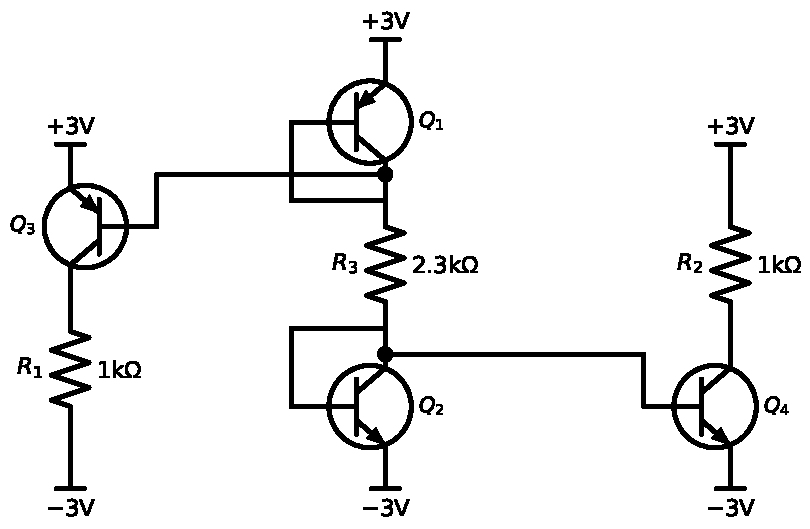
\includegraphics[width=0.9\linewidth,height=6cm,keepaspectratio]{p07_circuit}\end{center}
\solstep{1}{Assumptions}Assume every transistor is in the active region and that every base current is negligible ($I_B\approx0$, tool T1): then $|V_{BE}| = 0.7$\,V, $I_C\approx I_E$, and no current flows into any base, so a base network behaves like a plain resistor divider.
\solstep{2}{Walk through the circuit}\begin{enumerate}[leftmargin=*,itemsep=3pt]
\item $Q_{3}$ is active: $V_{B3} = 3 - 0.7 = 2.3\,\mathrm{V}$.
\item $Q_{2}$ (diode-connected) is active: $V_{B2} = (-3) + 0.7 = -2.3\,\mathrm{V}$.
\item KCL at the collector of $Q_{2}$ (base current neglected): \[I_{C2} = \frac{V_{B3} - V_{B2}}{R_{3}} = 2\,\mathrm{m}\mathrm{A}\]
\item KCL at the collector of $Q_{1}$ (base current neglected): \[I_{C1} = \frac{V_{B3} - V_{B2}}{R_{3}} = 2\,\mathrm{m}\mathrm{A}\]
\item $Q_{3}$ has the same base and emitter nodes as $Q_{1}$, hence the same $V_{BE}$ and the same current (current mirror): $I_{C3} = I_{C1} = 2\,\mathrm{m}\mathrm{A}$.
\item $Q_{4}$ has the same base and emitter nodes as $Q_{2}$, hence the same $V_{BE}$ and the same current (current mirror): $I_{C4} = I_{C2} = 2\,\mathrm{m}\mathrm{A}$.
\item The current $I_{C3} = 2\,\mathrm{m}\mathrm{A}$ flows from $V_{C3}$ through $R_{1}$: $V_{C3} = (-3) + R_{1}\,(I_{C3}) = -3 + 1\,\mathrm{k}\times2\,\mathrm{m}\mathrm{A} = -1\,\mathrm{V}$.
\item $Q_{4}$ draws $I_{C4} = 2\,\mathrm{m}\mathrm{A}$ from $V_{C4}$ through $R_{2}$: $V_{C4} = 3 - R_{2}\,(I_{C4}) = 3 - 1\,\mathrm{k}\times2\,\mathrm{m}\mathrm{A} = 1\,\mathrm{V}$.
\end{enumerate}

\solstep{3}{Verify the assumptions}\begin{itemize}[leftmargin=*,itemsep=2pt]
\item $I_{B3} = \frac{I_{C3}}{\beta} = 20\,\mu \mathrm{A}$ (all bases on this node: $40\,\mu \mathrm{A}$) $\ll$ the $2\,\mathrm{m}\mathrm{A}$ flowing in the base network \checkmark
\item $I_{B1} = \frac{I_{C1}}{\beta} = 20\,\mu \mathrm{A}$ (all bases on this node: $40\,\mu \mathrm{A}$) $\ll$ the $2\,\mathrm{m}\mathrm{A}$ flowing in the base network \checkmark
\item $I_{B2} = \frac{I_{C2}}{\beta} = 20\,\mu \mathrm{A}$ (all bases on this node: $40\,\mu \mathrm{A}$) $\ll$ the $2\,\mathrm{m}\mathrm{A}$ flowing in the base network \checkmark
\item $I_{B4} = \frac{I_{C4}}{\beta} = 20\,\mu \mathrm{A}$ (all bases on this node: $40\,\mu \mathrm{A}$) $\ll$ the $2\,\mathrm{m}\mathrm{A}$ flowing in the base network \checkmark
\item $V_{EC3} = 3 - V_{C3} = 3 - (-1) = 4\,\mathrm{V}$ $\ge 0.2$\,V $\Rightarrow$ $Q_{3}$ is active \checkmark
\item $V_{EC1} = 3 - V_{B3} = 3 - (2.3) = 0.7\,\mathrm{V}$ $\ge 0.2$\,V $\Rightarrow$ $Q_{1}$ is active \checkmark
\item $V_{CE2} = V_{B2} - (-3) = -2.3 - (-3) = 0.7\,\mathrm{V}$ $\ge 0.2$\,V $\Rightarrow$ $Q_{2}$ is active \checkmark
\item $V_{CE4} = V_{C4} - (-3) = 1 - (-3) = 4\,\mathrm{V}$ $\ge 0.2$\,V $\Rightarrow$ $Q_{4}$ is active \checkmark
\end{itemize}

\solstep{4}{How good was $I_B\approx 0$?}If we keep the base currents ($I_C=\beta I_B$ with $\beta=100$) and solve the circuit exactly, the currents change only a little:\begin{center}\renewcommand{\arraystretch}{1.35}
\begin{tabular}{cccc}
\toprule
transistor & $I_C$ (with $I_B\approx0$) & $I_C$ (exact) & difference \\
\midrule
$Q_{3}$ & $2\,\mathrm{m}\mathrm{A}$ & $1.96\,\mathrm{m}\mathrm{A}$ & $2\%$ \\
$Q_{1}$ & $2\,\mathrm{m}\mathrm{A}$ & $1.96\,\mathrm{m}\mathrm{A}$ & $2\%$ \\
$Q_{2}$ & $2\,\mathrm{m}\mathrm{A}$ & $1.96\,\mathrm{m}\mathrm{A}$ & $2\%$ \\
$Q_{4}$ & $2\,\mathrm{m}\mathrm{A}$ & $1.96\,\mathrm{m}\mathrm{A}$ & $2\%$ \\
\bottomrule
\end{tabular}\end{center}

\begin{ansbox}
$I_{C3} = 2\,\mathrm{m}\mathrm{A}$,\quad $I_{C1} = 2\,\mathrm{m}\mathrm{A}$,\quad $I_{C2} = 2\,\mathrm{m}\mathrm{A}$,\quad $I_{C4} = 2\,\mathrm{m}\mathrm{A}$\\[2pt] all transistors active, all base currents negligible.
\end{ansbox}

\newpage
\subsection*{Solution 4B.8 \hfill Medium}
\begin{center}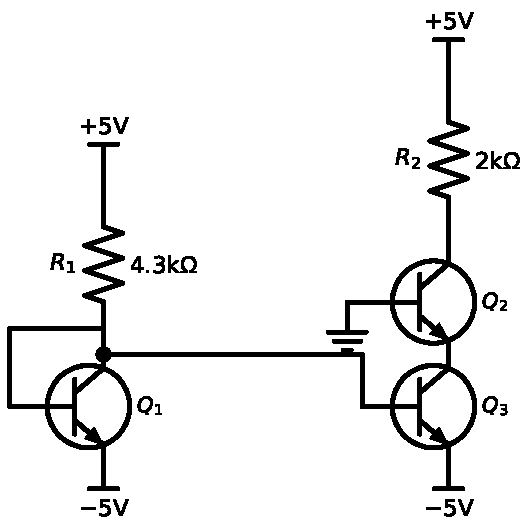
\includegraphics[width=0.9\linewidth,height=6cm,keepaspectratio]{p08_circuit}\end{center}
\solstep{1}{Assumptions}Assume every transistor is in the active region and that every base current is negligible ($I_B\approx0$, tool T1): then $|V_{BE}| = 0.7$\,V, $I_C\approx I_E$, and no current flows into any base, so a base network behaves like a plain resistor divider.
\solstep{2}{Walk through the circuit}\begin{enumerate}[leftmargin=*,itemsep=3pt]
\item $Q_{1}$ (diode-connected) is active: $V_{B1} = (-5) + 0.7 = -4.3\,\mathrm{V}$.
\item $Q_{2}$ is npn and assumed active: $V_{BE} = 0.7$\,V, so $V_{E2} = 0 - 0.7 = -0.7\,\mathrm{V}$.
\item KCL at the collector of $Q_{1}$ (base current neglected): \[I_{C1} = \frac{5 - V_{B1}}{R_{1}} = 2.16\,\mathrm{m}\mathrm{A}\]
\item $Q_{3}$ has the same base and emitter nodes as $Q_{1}$, hence the same $V_{BE}$ and the same current (current mirror): $I_{C3} = I_{C1} = 2.16\,\mathrm{m}\mathrm{A}$.
\item KCL at the emitter of $Q_{2}$ (base current neglected): \[I_{E2} = I_{C3} = 2.16\,\mathrm{m}\mathrm{A}, \qquad I_{C2} \approx I_{E2}\]
\item $Q_{2}$ draws $I_{C2} = 2.16\,\mathrm{m}\mathrm{A}$ from $V_{C2}$ through $R_{2}$: $V_{C2} = 5 - R_{2}\,(I_{C2}) = 5 - 2\,\mathrm{k}\times2.16\,\mathrm{m}\mathrm{A} = 0.674\,\mathrm{V}$.
\end{enumerate}

\solstep{3}{Verify the assumptions}\begin{itemize}[leftmargin=*,itemsep=2pt]
\item $I_{B1} = \frac{I_{C1}}{\beta} = 21.6\,\mu \mathrm{A}$ (all bases on this node: $43.3\,\mu \mathrm{A}$) $\ll$ the $2.16\,\mathrm{m}\mathrm{A}$ flowing in the base network \checkmark
\item $I_{B3} = \frac{I_{C3}}{\beta} = 21.6\,\mu \mathrm{A}$ (all bases on this node: $43.3\,\mu \mathrm{A}$) $\ll$ the $2.16\,\mathrm{m}\mathrm{A}$ flowing in the base network \checkmark
\item $V_{CE1} = V_{B1} - (-5) = -4.3 - (-5) = 0.7\,\mathrm{V}$ $\ge 0.2$\,V $\Rightarrow$ $Q_{1}$ is active \checkmark
\item $V_{CE2} = V_{C2} - V_{E2} = 0.6744 - (-0.7) = 1.37\,\mathrm{V}$ $\ge 0.2$\,V $\Rightarrow$ $Q_{2}$ is active \checkmark
\item $V_{CE3} = V_{E2} - (-5) = -0.7 - (-5) = 4.3\,\mathrm{V}$ $\ge 0.2$\,V $\Rightarrow$ $Q_{3}$ is active \checkmark
\end{itemize}

\solstep{4}{How good was $I_B\approx 0$?}If we keep the base currents ($I_C=\beta I_B$ with $\beta=100$) and solve the circuit exactly, the currents change only a little:\begin{center}\renewcommand{\arraystretch}{1.35}
\begin{tabular}{cccc}
\toprule
transistor & $I_C$ (with $I_B\approx0$) & $I_C$ (exact) & difference \\
\midrule
$Q_{1}$ & $2.16\,\mathrm{m}\mathrm{A}$ & $2.12\,\mathrm{m}\mathrm{A}$ & $2\%$ \\
$Q_{2}$ & $2.16\,\mathrm{m}\mathrm{A}$ & $2.1\,\mathrm{m}\mathrm{A}$ & $3\%$ \\
$Q_{3}$ & $2.16\,\mathrm{m}\mathrm{A}$ & $2.12\,\mathrm{m}\mathrm{A}$ & $2\%$ \\
\bottomrule
\end{tabular}\end{center}

\begin{ansbox}
$I_{C1} = 2.16\,\mathrm{m}\mathrm{A}$,\quad $I_{C2} = 2.16\,\mathrm{m}\mathrm{A}$,\quad $I_{C3} = 2.16\,\mathrm{m}\mathrm{A}$\\[2pt] all transistors active, all base currents negligible.
\end{ansbox}

\newpage
\subsection*{Solution 4B.9 \hfill Medium}
\begin{center}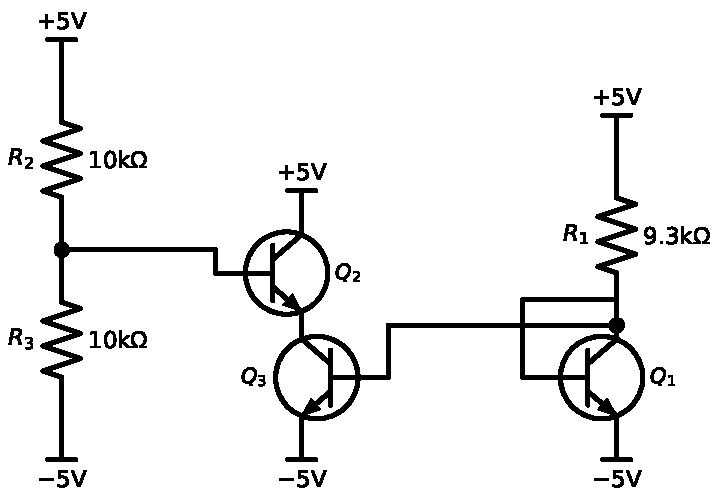
\includegraphics[width=0.9\linewidth,height=6cm,keepaspectratio]{p09_circuit}\end{center}
\solstep{1}{Assumptions}Assume every transistor is in the active region and that every base current is negligible ($I_B\approx0$, tool T1): then $|V_{BE}| = 0.7$\,V, $I_C\approx I_E$, and no current flows into any base, so a base network behaves like a plain resistor divider.
\solstep{2}{Walk through the circuit}\begin{enumerate}[leftmargin=*,itemsep=3pt]
\item $Q_{3}$ is active: $V_{B3} = (-5) + 0.7 = -4.3\,\mathrm{V}$.
\item No current flows into the base ($I_B$ is negligible), so $V_{B2}$ is set by the divider $R_{2}$--$R_{3}$ between $5$ and $(-5)$ (Lecture-1 tool):\[V_{B2} = -5 + (5 - (-5))\frac{10\,\mathrm{k}}{10\,\mathrm{k} + 10\,\mathrm{k}} = 0\,\mathrm{V}\]
\item KCL at the collector of $Q_{1}$ (base current neglected): \[I_{C1} = \frac{5 - V_{B3}}{R_{1}} = 1\,\mathrm{m}\mathrm{A}\]
\item $Q_{2}$ is npn and assumed active: $V_{BE} = 0.7$\,V, so $V_{E2} = V_{B2} - 0.7 = -0.7\,\mathrm{V}$.
\item $Q_{3}$ has the same base and emitter nodes as $Q_{1}$, hence the same $V_{BE}$ and the same current (current mirror): $I_{C3} = I_{C1} = 1\,\mathrm{m}\mathrm{A}$.
\item KCL at the emitter of $Q_{2}$ (base current neglected): \[I_{E2} = I_{C3} = 1\,\mathrm{m}\mathrm{A}, \qquad I_{C2} \approx I_{E2}\]
\end{enumerate}

\solstep{3}{Verify the assumptions}\begin{itemize}[leftmargin=*,itemsep=2pt]
\item $I_{B2} = \frac{I_{C2}}{\beta} = 10\,\mu \mathrm{A}$ $\ll$ the $500\,\mu \mathrm{A}$ flowing in the base network \checkmark
\item $I_{B3} = \frac{I_{C3}}{\beta} = 10\,\mu \mathrm{A}$ (all bases on this node: $20\,\mu \mathrm{A}$) $\ll$ the $1\,\mathrm{m}\mathrm{A}$ flowing in the base network \checkmark
\item $I_{B1} = \frac{I_{C1}}{\beta} = 10\,\mu \mathrm{A}$ (all bases on this node: $20\,\mu \mathrm{A}$) $\ll$ the $1\,\mathrm{m}\mathrm{A}$ flowing in the base network \checkmark
\item $V_{CE2} = 5 - V_{E2} = 5 - (-0.7) = 5.7\,\mathrm{V}$ $\ge 0.2$\,V $\Rightarrow$ $Q_{2}$ is active \checkmark
\item $V_{CE3} = V_{E2} - (-5) = -0.7 - (-5) = 4.3\,\mathrm{V}$ $\ge 0.2$\,V $\Rightarrow$ $Q_{3}$ is active \checkmark
\item $V_{CE1} = V_{B3} - (-5) = -4.3 - (-5) = 0.7\,\mathrm{V}$ $\ge 0.2$\,V $\Rightarrow$ $Q_{1}$ is active \checkmark
\end{itemize}

\solstep{4}{How good was $I_B\approx 0$?}If we keep the base currents ($I_C=\beta I_B$ with $\beta=100$) and solve the circuit exactly, the currents change only a little:\begin{center}\renewcommand{\arraystretch}{1.35}
\begin{tabular}{cccc}
\toprule
transistor & $I_C$ (with $I_B\approx0$) & $I_C$ (exact) & difference \\
\midrule
$Q_{2}$ & $1\,\mathrm{m}\mathrm{A}$ & $971\,\mu \mathrm{A}$ & $3\%$ \\
$Q_{3}$ & $1\,\mathrm{m}\mathrm{A}$ & $980\,\mu \mathrm{A}$ & $2\%$ \\
$Q_{1}$ & $1\,\mathrm{m}\mathrm{A}$ & $980\,\mu \mathrm{A}$ & $2\%$ \\
\bottomrule
\end{tabular}\end{center}

\begin{ansbox}
$I_{C2} = 1\,\mathrm{m}\mathrm{A}$,\quad $I_{C3} = 1\,\mathrm{m}\mathrm{A}$,\quad $I_{C1} = 1\,\mathrm{m}\mathrm{A}$\\[2pt] all transistors active, all base currents negligible.
\end{ansbox}

\newpage
\subsection*{Solution 4B.10 \hfill Medium}
\begin{center}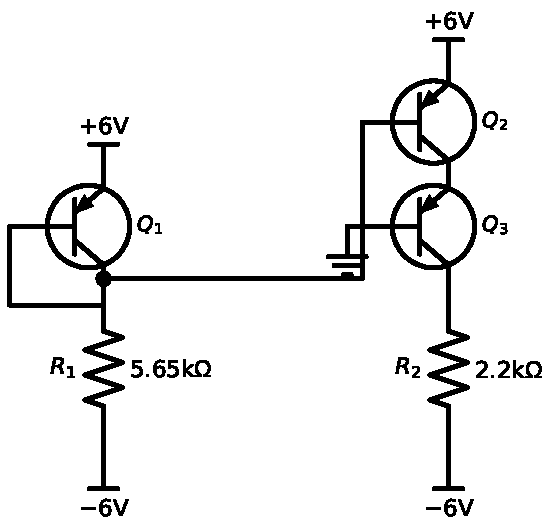
\includegraphics[width=0.9\linewidth,height=6cm,keepaspectratio]{p10_circuit}\end{center}
\solstep{1}{Assumptions}Assume every transistor is in the active region and that every base current is negligible ($I_B\approx0$, tool T1): then $|V_{BE}| = 0.7$\,V, $I_C\approx I_E$, and no current flows into any base, so a base network behaves like a plain resistor divider.
\solstep{2}{Walk through the circuit}\begin{enumerate}[leftmargin=*,itemsep=3pt]
\item $Q_{1}$ (diode-connected) is active: $V_{B1} = 6 - 0.7 = 5.3\,\mathrm{V}$.
\item $Q_{3}$ is pnp and assumed active: $V_{BE} = -0.7$\,V, so $V_{C2} = 0 + 0.7 = 0.7\,\mathrm{V}$.
\item KCL at the collector of $Q_{1}$ (base current neglected): \[I_{C1} = \frac{V_{B1} - (-6)}{R_{1}} = 2\,\mathrm{m}\mathrm{A}\]
\item $Q_{2}$ has the same base and emitter nodes as $Q_{1}$, hence the same $V_{BE}$ and the same current (current mirror): $I_{C2} = I_{C1} = 2\,\mathrm{m}\mathrm{A}$.
\item KCL at the emitter of $Q_{3}$ (base current neglected): \[I_{E3} = I_{C2} = 2\,\mathrm{m}\mathrm{A}, \qquad I_{C3} \approx I_{E3}\]
\item The current $I_{C3} = 2\,\mathrm{m}\mathrm{A}$ flows from $V_{C3}$ through $R_{2}$: $V_{C3} = (-6) + R_{2}\,(I_{C3}) = -6 + 2.2\,\mathrm{k}\times2\,\mathrm{m}\mathrm{A} = -1.6\,\mathrm{V}$.
\end{enumerate}

\solstep{3}{Verify the assumptions}\begin{itemize}[leftmargin=*,itemsep=2pt]
\item $I_{B1} = \frac{I_{C1}}{\beta} = 20\,\mu \mathrm{A}$ (all bases on this node: $40\,\mu \mathrm{A}$) $\ll$ the $2\,\mathrm{m}\mathrm{A}$ flowing in the base network \checkmark
\item $I_{B2} = \frac{I_{C2}}{\beta} = 20\,\mu \mathrm{A}$ (all bases on this node: $40\,\mu \mathrm{A}$) $\ll$ the $2\,\mathrm{m}\mathrm{A}$ flowing in the base network \checkmark
\item $V_{EC1} = 6 - V_{B1} = 6 - (5.3) = 0.7\,\mathrm{V}$ $\ge 0.2$\,V $\Rightarrow$ $Q_{1}$ is active \checkmark
\item $V_{EC2} = 6 - V_{C2} = 6 - (0.7) = 5.3\,\mathrm{V}$ $\ge 0.2$\,V $\Rightarrow$ $Q_{2}$ is active \checkmark
\item $V_{EC3} = V_{C2} - V_{C3} = 0.7 - (-1.6) = 2.3\,\mathrm{V}$ $\ge 0.2$\,V $\Rightarrow$ $Q_{3}$ is active \checkmark
\end{itemize}

\solstep{4}{How good was $I_B\approx 0$?}If we keep the base currents ($I_C=\beta I_B$ with $\beta=100$) and solve the circuit exactly, the currents change only a little:\begin{center}\renewcommand{\arraystretch}{1.35}
\begin{tabular}{cccc}
\toprule
transistor & $I_C$ (with $I_B\approx0$) & $I_C$ (exact) & difference \\
\midrule
$Q_{1}$ & $2\,\mathrm{m}\mathrm{A}$ & $1.96\,\mathrm{m}\mathrm{A}$ & $2\%$ \\
$Q_{2}$ & $2\,\mathrm{m}\mathrm{A}$ & $1.96\,\mathrm{m}\mathrm{A}$ & $2\%$ \\
$Q_{3}$ & $2\,\mathrm{m}\mathrm{A}$ & $1.94\,\mathrm{m}\mathrm{A}$ & $3\%$ \\
\bottomrule
\end{tabular}\end{center}

\begin{ansbox}
$I_{C1} = 2\,\mathrm{m}\mathrm{A}$,\quad $I_{C2} = 2\,\mathrm{m}\mathrm{A}$,\quad $I_{C3} = 2\,\mathrm{m}\mathrm{A}$\\[2pt] all transistors active, all base currents negligible.
\end{ansbox}

\newpage
\subsection*{Solution 4B.11 \hfill Medium}
\begin{center}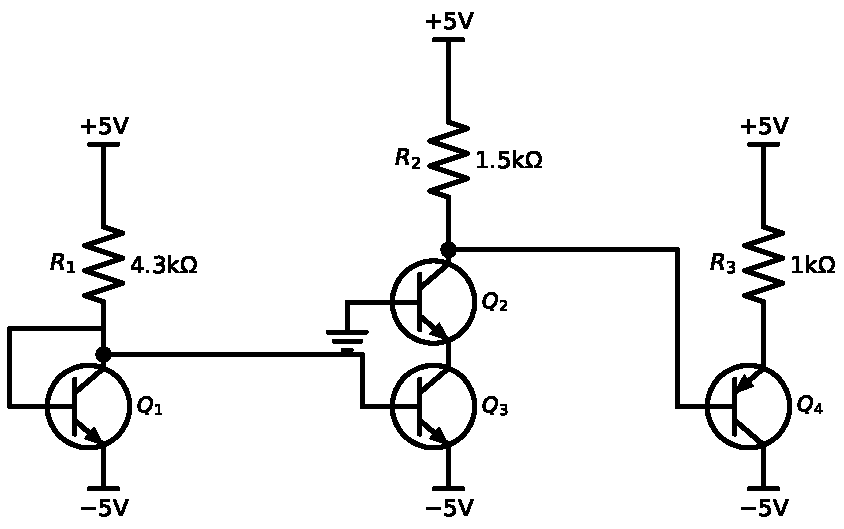
\includegraphics[width=0.9\linewidth,height=6cm,keepaspectratio]{p11_circuit}\end{center}
\solstep{1}{Assumptions}Assume every transistor is in the active region and that every base current is negligible ($I_B\approx0$, tool T1): then $|V_{BE}| = 0.7$\,V, $I_C\approx I_E$, and no current flows into any base, so a base network behaves like a plain resistor divider.
\solstep{2}{Walk through the circuit}\begin{enumerate}[leftmargin=*,itemsep=3pt]
\item $Q_{1}$ (diode-connected) is active: $V_{B1} = (-5) + 0.7 = -4.3\,\mathrm{V}$.
\item $Q_{2}$ is npn and assumed active: $V_{BE} = 0.7$\,V, so $V_{E2} = 0 - 0.7 = -0.7\,\mathrm{V}$.
\item KCL at the collector of $Q_{1}$ (base current neglected): \[I_{C1} = \frac{5 - V_{B1}}{R_{1}} = 2.16\,\mathrm{m}\mathrm{A}\]
\item $Q_{3}$ has the same base and emitter nodes as $Q_{1}$, hence the same $V_{BE}$ and the same current (current mirror): $I_{C3} = I_{C1} = 2.16\,\mathrm{m}\mathrm{A}$.
\item KCL at the emitter of $Q_{2}$ (base current neglected): \[I_{E2} = I_{C3} = 2.16\,\mathrm{m}\mathrm{A}, \qquad I_{C2} \approx I_{E2}\]
\item $Q_{2}$ draws $I_{C2} = 2.16\,\mathrm{m}\mathrm{A}$ from $V_{C2}$ through $R_{2}$: $V_{C2} = 5 - R_{2}\,(I_{C2}) = 5 - 1.5\,\mathrm{k}\times2.16\,\mathrm{m}\mathrm{A} = 1.76\,\mathrm{V}$.
\item $Q_{4}$ is pnp and assumed active: $V_{BE} = -0.7$\,V, so $V_{E4} = V_{C2} + 0.7 = 2.46\,\mathrm{V}$.
\item KCL at the emitter of $Q_{4}$ (base current neglected): \[I_{E4} = \frac{5 - V_{E4}}{R_{3}} = 2.54\,\mathrm{m}\mathrm{A}, \qquad I_{C4} \approx I_{E4}\]
\end{enumerate}

\solstep{3}{Verify the assumptions}\begin{itemize}[leftmargin=*,itemsep=2pt]
\item $I_{B1} = \frac{I_{C1}}{\beta} = 21.6\,\mu \mathrm{A}$ (all bases on this node: $43.3\,\mu \mathrm{A}$) $\ll$ the $2.16\,\mathrm{m}\mathrm{A}$ flowing in the base network \checkmark
\item $I_{B3} = \frac{I_{C3}}{\beta} = 21.6\,\mu \mathrm{A}$ (all bases on this node: $43.3\,\mu \mathrm{A}$) $\ll$ the $2.16\,\mathrm{m}\mathrm{A}$ flowing in the base network \checkmark
\item $I_{B4} = \frac{I_{C4}}{\beta} = 25.4\,\mu \mathrm{A}$ $\ll$ the $2.16\,\mathrm{m}\mathrm{A}$ flowing in the base network \checkmark
\item $V_{CE1} = V_{B1} - (-5) = -4.3 - (-5) = 0.7\,\mathrm{V}$ $\ge 0.2$\,V $\Rightarrow$ $Q_{1}$ is active \checkmark
\item $V_{CE2} = V_{C2} - V_{E2} = 1.756 - (-0.7) = 2.46\,\mathrm{V}$ $\ge 0.2$\,V $\Rightarrow$ $Q_{2}$ is active \checkmark
\item $V_{CE3} = V_{E2} - (-5) = -0.7 - (-5) = 4.3\,\mathrm{V}$ $\ge 0.2$\,V $\Rightarrow$ $Q_{3}$ is active \checkmark
\item $V_{EC4} = V_{E4} - (-5) = 2.456 - (-5) = 7.46\,\mathrm{V}$ $\ge 0.2$\,V $\Rightarrow$ $Q_{4}$ is active \checkmark
\end{itemize}

\solstep{4}{How good was $I_B\approx 0$?}If we keep the base currents ($I_C=\beta I_B$ with $\beta=100$) and solve the circuit exactly, the currents change only a little:\begin{center}\renewcommand{\arraystretch}{1.35}
\begin{tabular}{cccc}
\toprule
transistor & $I_C$ (with $I_B\approx0$) & $I_C$ (exact) & difference \\
\midrule
$Q_{1}$ & $2.16\,\mathrm{m}\mathrm{A}$ & $2.12\,\mathrm{m}\mathrm{A}$ & $2\%$ \\
$Q_{2}$ & $2.16\,\mathrm{m}\mathrm{A}$ & $2.1\,\mathrm{m}\mathrm{A}$ & $3\%$ \\
$Q_{3}$ & $2.16\,\mathrm{m}\mathrm{A}$ & $2.12\,\mathrm{m}\mathrm{A}$ & $2\%$ \\
$Q_{4}$ & $2.54\,\mathrm{m}\mathrm{A}$ & $2.39\,\mathrm{m}\mathrm{A}$ & $6.5\%$ \\
\bottomrule
\end{tabular}\end{center}
 The differences grow along the chain: every base current slightly shifts the collector voltage that biases the next transistor, and $\alpha = \beta/(\beta+1)$ makes each $I_C$ about 1\,\% smaller than its $I_E$. A shift is amplified when the next stage has only a small voltage across its emitter resistor. Hand analysis with $I_B\approx0$ is still the standard first pass.
\begin{ansbox}
$I_{C1} = 2.16\,\mathrm{m}\mathrm{A}$,\quad $I_{C2} = 2.16\,\mathrm{m}\mathrm{A}$,\quad $I_{C3} = 2.16\,\mathrm{m}\mathrm{A}$,\quad $I_{C4} = 2.54\,\mathrm{m}\mathrm{A}$\\[2pt] all transistors active, all base currents negligible.
\end{ansbox}

\newpage
\subsection*{Solution 4B.12 \hfill Medium}
\begin{center}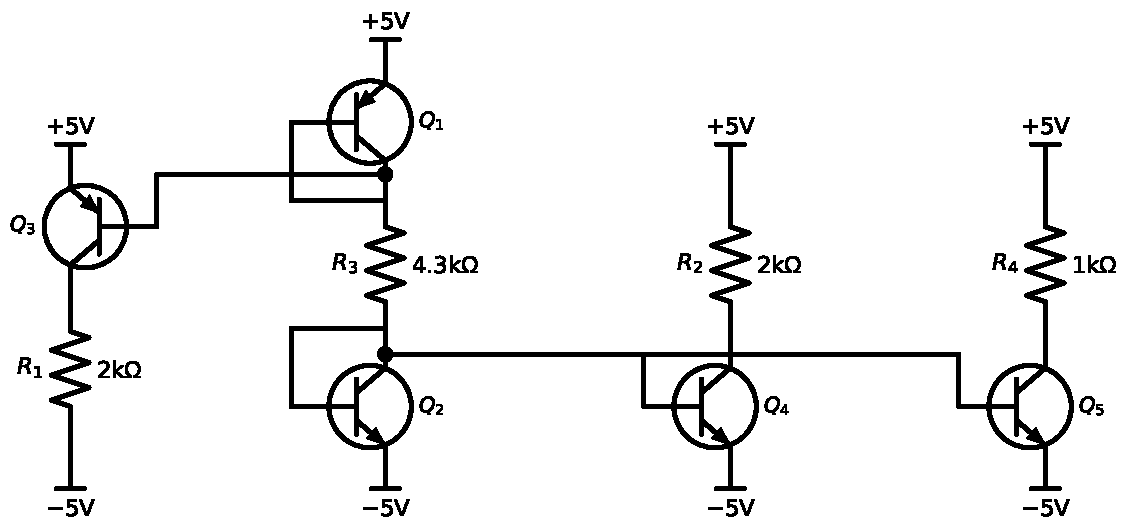
\includegraphics[width=0.9\linewidth,height=6cm,keepaspectratio]{p12_circuit}\end{center}
\solstep{1}{Assumptions}Assume every transistor is in the active region and that every base current is negligible ($I_B\approx0$, tool T1): then $|V_{BE}| = 0.7$\,V, $I_C\approx I_E$, and no current flows into any base, so a base network behaves like a plain resistor divider.
\solstep{2}{Walk through the circuit}\begin{enumerate}[leftmargin=*,itemsep=3pt]
\item $Q_{3}$ is active: $V_{B3} = 5 - 0.7 = 4.3\,\mathrm{V}$.
\item $Q_{2}$ (diode-connected) is active: $V_{B2} = (-5) + 0.7 = -4.3\,\mathrm{V}$.
\item KCL at the collector of $Q_{2}$ (base current neglected): \[I_{C2} = \frac{V_{B3} - V_{B2}}{R_{3}} = 2\,\mathrm{m}\mathrm{A}\]
\item KCL at the collector of $Q_{1}$ (base current neglected): \[I_{C1} = \frac{V_{B3} - V_{B2}}{R_{3}} = 2\,\mathrm{m}\mathrm{A}\]
\item $Q_{3}$ has the same base and emitter nodes as $Q_{1}$, hence the same $V_{BE}$ and the same current (current mirror): $I_{C3} = I_{C1} = 2\,\mathrm{m}\mathrm{A}$.
\item $Q_{4}$ has the same base and emitter nodes as $Q_{2}$, hence the same $V_{BE}$ and the same current (current mirror): $I_{C4} = I_{C2} = 2\,\mathrm{m}\mathrm{A}$.
\item $Q_{5}$ has the same base and emitter nodes as $Q_{2}$, hence the same $V_{BE}$ and the same current (current mirror): $I_{C5} = I_{C2} = 2\,\mathrm{m}\mathrm{A}$.
\item The current $I_{C3} = 2\,\mathrm{m}\mathrm{A}$ flows from $V_{C3}$ through $R_{1}$: $V_{C3} = (-5) + R_{1}\,(I_{C3}) = -5 + 2\,\mathrm{k}\times2\,\mathrm{m}\mathrm{A} = -1\,\mathrm{V}$.
\item $Q_{4}$ draws $I_{C4} = 2\,\mathrm{m}\mathrm{A}$ from $V_{C4}$ through $R_{2}$: $V_{C4} = 5 - R_{2}\,(I_{C4}) = 5 - 2\,\mathrm{k}\times2\,\mathrm{m}\mathrm{A} = 1\,\mathrm{V}$.
\item $Q_{5}$ draws $I_{C5} = 2\,\mathrm{m}\mathrm{A}$ from $V_{C5}$ through $R_{4}$: $V_{C5} = 5 - R_{4}\,(I_{C5}) = 5 - 1\,\mathrm{k}\times2\,\mathrm{m}\mathrm{A} = 3\,\mathrm{V}$.
\end{enumerate}

\solstep{3}{Verify the assumptions}\begin{itemize}[leftmargin=*,itemsep=2pt]
\item $I_{B3} = \frac{I_{C3}}{\beta} = 20\,\mu \mathrm{A}$ (all bases on this node: $40\,\mu \mathrm{A}$) $\ll$ the $2\,\mathrm{m}\mathrm{A}$ flowing in the base network \checkmark
\item $I_{B1} = \frac{I_{C1}}{\beta} = 20\,\mu \mathrm{A}$ (all bases on this node: $40\,\mu \mathrm{A}$) $\ll$ the $2\,\mathrm{m}\mathrm{A}$ flowing in the base network \checkmark
\item $I_{B2} = \frac{I_{C2}}{\beta} = 20\,\mu \mathrm{A}$ (all bases on this node: $60\,\mu \mathrm{A}$) $\ll$ the $2\,\mathrm{m}\mathrm{A}$ flowing in the base network \checkmark
\item $I_{B4} = \frac{I_{C4}}{\beta} = 20\,\mu \mathrm{A}$ (all bases on this node: $60\,\mu \mathrm{A}$) $\ll$ the $2\,\mathrm{m}\mathrm{A}$ flowing in the base network \checkmark
\item $I_{B5} = \frac{I_{C5}}{\beta} = 20\,\mu \mathrm{A}$ (all bases on this node: $60\,\mu \mathrm{A}$) $\ll$ the $2\,\mathrm{m}\mathrm{A}$ flowing in the base network \checkmark
\item $V_{EC3} = 5 - V_{C3} = 5 - (-1) = 6\,\mathrm{V}$ $\ge 0.2$\,V $\Rightarrow$ $Q_{3}$ is active \checkmark
\item $V_{EC1} = 5 - V_{B3} = 5 - (4.3) = 0.7\,\mathrm{V}$ $\ge 0.2$\,V $\Rightarrow$ $Q_{1}$ is active \checkmark
\item $V_{CE2} = V_{B2} - (-5) = -4.3 - (-5) = 0.7\,\mathrm{V}$ $\ge 0.2$\,V $\Rightarrow$ $Q_{2}$ is active \checkmark
\item $V_{CE4} = V_{C4} - (-5) = 1 - (-5) = 6\,\mathrm{V}$ $\ge 0.2$\,V $\Rightarrow$ $Q_{4}$ is active \checkmark
\item $V_{CE5} = V_{C5} - (-5) = 3 - (-5) = 8\,\mathrm{V}$ $\ge 0.2$\,V $\Rightarrow$ $Q_{5}$ is active \checkmark
\end{itemize}

\solstep{4}{How good was $I_B\approx 0$?}If we keep the base currents ($I_C=\beta I_B$ with $\beta=100$) and solve the circuit exactly, the currents change only a little:\begin{center}\renewcommand{\arraystretch}{1.35}
\begin{tabular}{cccc}
\toprule
transistor & $I_C$ (with $I_B\approx0$) & $I_C$ (exact) & difference \\
\midrule
$Q_{3}$ & $2\,\mathrm{m}\mathrm{A}$ & $1.96\,\mathrm{m}\mathrm{A}$ & $2\%$ \\
$Q_{1}$ & $2\,\mathrm{m}\mathrm{A}$ & $1.96\,\mathrm{m}\mathrm{A}$ & $2\%$ \\
$Q_{2}$ & $2\,\mathrm{m}\mathrm{A}$ & $1.94\,\mathrm{m}\mathrm{A}$ & $3\%$ \\
$Q_{4}$ & $2\,\mathrm{m}\mathrm{A}$ & $1.94\,\mathrm{m}\mathrm{A}$ & $3\%$ \\
$Q_{5}$ & $2\,\mathrm{m}\mathrm{A}$ & $1.94\,\mathrm{m}\mathrm{A}$ & $3\%$ \\
\bottomrule
\end{tabular}\end{center}

\begin{ansbox}
$I_{C3} = 2\,\mathrm{m}\mathrm{A}$,\quad $I_{C1} = 2\,\mathrm{m}\mathrm{A}$,\quad $I_{C2} = 2\,\mathrm{m}\mathrm{A}$,\quad $I_{C4} = 2\,\mathrm{m}\mathrm{A}$,\quad $I_{C5} = 2\,\mathrm{m}\mathrm{A}$\\[2pt] all transistors active, all base currents negligible.
\end{ansbox}

\newpage
\subsection*{Solution 4B.13 \hfill Hard}
\begin{center}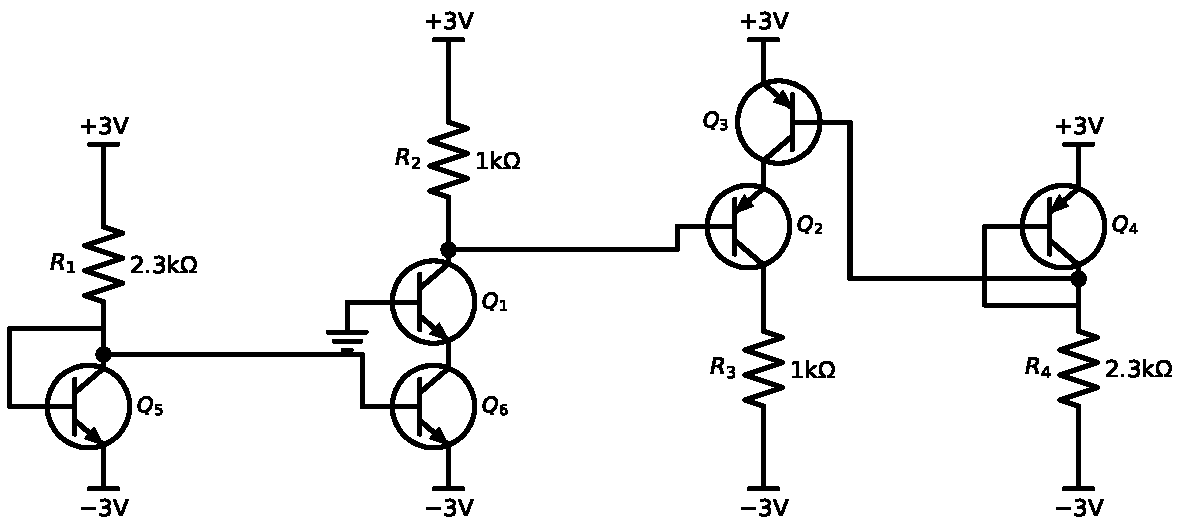
\includegraphics[width=0.9\linewidth,height=6cm,keepaspectratio]{p13_circuit}\end{center}
\solstep{1}{Assumptions}Assume every transistor is in the active region and that every base current is negligible ($I_B\approx0$, tool T1): then $|V_{BE}| = 0.7$\,V, $I_C\approx I_E$, and no current flows into any base, so a base network behaves like a plain resistor divider.
\solstep{2}{Walk through the circuit}\begin{enumerate}[leftmargin=*,itemsep=3pt]
\item $Q_{5}$ (diode-connected) is active: $V_{B5} = (-3) + 0.7 = -2.3\,\mathrm{V}$.
\item $Q_{1}$ is npn and assumed active: $V_{BE} = 0.7$\,V, so $V_{E1} = 0 - 0.7 = -0.7\,\mathrm{V}$.
\item $Q_{3}$ is active: $V_{B3} = 3 - 0.7 = 2.3\,\mathrm{V}$.
\item KCL at the collector of $Q_{5}$ (base current neglected): \[I_{C5} = \frac{3 - V_{B5}}{R_{1}} = 2.3\,\mathrm{m}\mathrm{A}\]
\item KCL at the collector of $Q_{4}$ (base current neglected): \[I_{C4} = \frac{V_{B3} - (-3)}{R_{4}} = 2.3\,\mathrm{m}\mathrm{A}\]
\item $Q_{6}$ has the same base and emitter nodes as $Q_{5}$, hence the same $V_{BE}$ and the same current (current mirror): $I_{C6} = I_{C5} = 2.3\,\mathrm{m}\mathrm{A}$.
\item $Q_{3}$ has the same base and emitter nodes as $Q_{4}$, hence the same $V_{BE}$ and the same current (current mirror): $I_{C3} = I_{C4} = 2.3\,\mathrm{m}\mathrm{A}$.
\item KCL at the emitter of $Q_{1}$ (base current neglected): \[I_{E1} = I_{C6} = 2.3\,\mathrm{m}\mathrm{A}, \qquad I_{C1} \approx I_{E1}\]
\item $Q_{1}$ draws $I_{C1} = 2.3\,\mathrm{m}\mathrm{A}$ from $V_{C1}$ through $R_{2}$: $V_{C1} = 3 - R_{2}\,(I_{C1}) = 3 - 1\,\mathrm{k}\times2.3\,\mathrm{m}\mathrm{A} = 0.696\,\mathrm{V}$.
\item $Q_{2}$ is pnp and assumed active: $V_{BE} = -0.7$\,V, so $V_{C3} = V_{C1} + 0.7 = 1.4\,\mathrm{V}$.
\item KCL at the emitter of $Q_{2}$ (base current neglected): \[I_{E2} = I_{C3} = 2.3\,\mathrm{m}\mathrm{A}, \qquad I_{C2} \approx I_{E2}\]
\item The current $I_{C2} = 2.3\,\mathrm{m}\mathrm{A}$ flows from $V_{C2}$ through $R_{3}$: $V_{C2} = (-3) + R_{3}\,(I_{C2}) = -3 + 1\,\mathrm{k}\times2.3\,\mathrm{m}\mathrm{A} = -0.696\,\mathrm{V}$.
\end{enumerate}

\solstep{3}{Verify the assumptions}\begin{itemize}[leftmargin=*,itemsep=2pt]
\item $I_{B5} = \frac{I_{C5}}{\beta} = 23\,\mu \mathrm{A}$ (all bases on this node: $46.1\,\mu \mathrm{A}$) $\ll$ the $2.3\,\mathrm{m}\mathrm{A}$ flowing in the base network \checkmark
\item $I_{B6} = \frac{I_{C6}}{\beta} = 23\,\mu \mathrm{A}$ (all bases on this node: $46.1\,\mu \mathrm{A}$) $\ll$ the $2.3\,\mathrm{m}\mathrm{A}$ flowing in the base network \checkmark
\item $I_{B3} = \frac{I_{C3}}{\beta} = 23\,\mu \mathrm{A}$ (all bases on this node: $46.1\,\mu \mathrm{A}$) $\ll$ the $2.3\,\mathrm{m}\mathrm{A}$ flowing in the base network \checkmark
\item $I_{B2} = \frac{I_{C2}}{\beta} = 23\,\mu \mathrm{A}$ $\ll$ the $2.3\,\mathrm{m}\mathrm{A}$ flowing in the base network \checkmark
\item $I_{B4} = \frac{I_{C4}}{\beta} = 23\,\mu \mathrm{A}$ (all bases on this node: $46.1\,\mu \mathrm{A}$) $\ll$ the $2.3\,\mathrm{m}\mathrm{A}$ flowing in the base network \checkmark
\item $V_{CE5} = V_{B5} - (-3) = -2.3 - (-3) = 0.7\,\mathrm{V}$ $\ge 0.2$\,V $\Rightarrow$ $Q_{5}$ is active \checkmark
\item $V_{CE1} = V_{C1} - V_{E1} = 0.6957 - (-0.7) = 1.4\,\mathrm{V}$ $\ge 0.2$\,V $\Rightarrow$ $Q_{1}$ is active \checkmark
\item $V_{CE6} = V_{E1} - (-3) = -0.7 - (-3) = 2.3\,\mathrm{V}$ $\ge 0.2$\,V $\Rightarrow$ $Q_{6}$ is active \checkmark
\item $V_{EC3} = 3 - V_{C3} = 3 - (1.396) = 1.6\,\mathrm{V}$ $\ge 0.2$\,V $\Rightarrow$ $Q_{3}$ is active \checkmark
\item $V_{EC2} = V_{C3} - V_{C2} = 1.396 - (-0.6957) = 2.09\,\mathrm{V}$ $\ge 0.2$\,V $\Rightarrow$ $Q_{2}$ is active \checkmark
\item $V_{EC4} = 3 - V_{B3} = 3 - (2.3) = 0.7\,\mathrm{V}$ $\ge 0.2$\,V $\Rightarrow$ $Q_{4}$ is active \checkmark
\end{itemize}

\solstep{4}{How good was $I_B\approx 0$?}If we keep the base currents ($I_C=\beta I_B$ with $\beta=100$) and solve the circuit exactly, the currents change only a little:\begin{center}\renewcommand{\arraystretch}{1.35}
\begin{tabular}{cccc}
\toprule
transistor & $I_C$ (with $I_B\approx0$) & $I_C$ (exact) & difference \\
\midrule
$Q_{5}$ & $2.3\,\mathrm{m}\mathrm{A}$ & $2.26\,\mathrm{m}\mathrm{A}$ & $2\%$ \\
$Q_{1}$ & $2.3\,\mathrm{m}\mathrm{A}$ & $2.24\,\mathrm{m}\mathrm{A}$ & $3\%$ \\
$Q_{6}$ & $2.3\,\mathrm{m}\mathrm{A}$ & $2.26\,\mathrm{m}\mathrm{A}$ & $2\%$ \\
$Q_{3}$ & $2.3\,\mathrm{m}\mathrm{A}$ & $2.26\,\mathrm{m}\mathrm{A}$ & $2\%$ \\
$Q_{2}$ & $2.3\,\mathrm{m}\mathrm{A}$ & $2.24\,\mathrm{m}\mathrm{A}$ & $3\%$ \\
$Q_{4}$ & $2.3\,\mathrm{m}\mathrm{A}$ & $2.26\,\mathrm{m}\mathrm{A}$ & $2\%$ \\
\bottomrule
\end{tabular}\end{center}

\begin{ansbox}
$I_{C5} = 2.3\,\mathrm{m}\mathrm{A}$,\quad $I_{C1} = 2.3\,\mathrm{m}\mathrm{A}$,\quad $I_{C6} = 2.3\,\mathrm{m}\mathrm{A}$,\quad $I_{C3} = 2.3\,\mathrm{m}\mathrm{A}$,\quad $I_{C2} = 2.3\,\mathrm{m}\mathrm{A}$,\quad $I_{C4} = 2.3\,\mathrm{m}\mathrm{A}$\\[2pt] all transistors active, all base currents negligible.
\end{ansbox}

\newpage
\subsection*{Solution 4B.14 \hfill Hard}
\begin{center}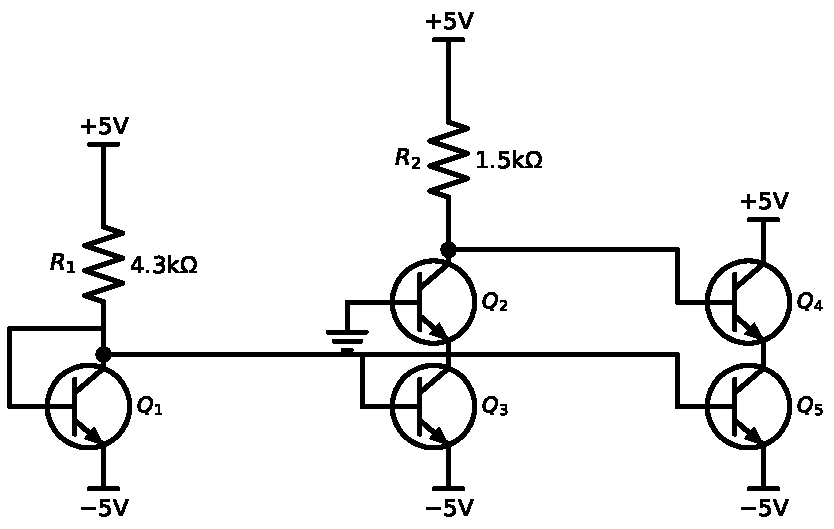
\includegraphics[width=0.9\linewidth,height=6cm,keepaspectratio]{p14_circuit}\end{center}
\solstep{1}{Assumptions}Assume every transistor is in the active region and that every base current is negligible ($I_B\approx0$, tool T1): then $|V_{BE}| = 0.7$\,V, $I_C\approx I_E$, and no current flows into any base, so a base network behaves like a plain resistor divider.
\solstep{2}{Walk through the circuit}\begin{enumerate}[leftmargin=*,itemsep=3pt]
\item $Q_{1}$ (diode-connected) is active: $V_{B1} = (-5) + 0.7 = -4.3\,\mathrm{V}$.
\item $Q_{2}$ is npn and assumed active: $V_{BE} = 0.7$\,V, so $V_{E2} = 0 - 0.7 = -0.7\,\mathrm{V}$.
\item KCL at the collector of $Q_{1}$ (base current neglected): \[I_{C1} = \frac{5 - V_{B1}}{R_{1}} = 2.16\,\mathrm{m}\mathrm{A}\]
\item $Q_{3}$ has the same base and emitter nodes as $Q_{1}$, hence the same $V_{BE}$ and the same current (current mirror): $I_{C3} = I_{C1} = 2.16\,\mathrm{m}\mathrm{A}$.
\item $Q_{5}$ has the same base and emitter nodes as $Q_{1}$, hence the same $V_{BE}$ and the same current (current mirror): $I_{C5} = I_{C1} = 2.16\,\mathrm{m}\mathrm{A}$.
\item KCL at the emitter of $Q_{2}$ (base current neglected): \[I_{E2} = I_{C3} = 2.16\,\mathrm{m}\mathrm{A}, \qquad I_{C2} \approx I_{E2}\]
\item $Q_{2}$ draws $I_{C2} = 2.16\,\mathrm{m}\mathrm{A}$ from $V_{C2}$ through $R_{2}$: $V_{C2} = 5 - R_{2}\,(I_{C2}) = 5 - 1.5\,\mathrm{k}\times2.16\,\mathrm{m}\mathrm{A} = 1.76\,\mathrm{V}$.
\item $Q_{4}$ is npn and assumed active: $V_{BE} = 0.7$\,V, so $V_{E4} = V_{C2} - 0.7 = 1.06\,\mathrm{V}$.
\item KCL at the emitter of $Q_{4}$ (base current neglected): \[I_{E4} = I_{C5} = 2.16\,\mathrm{m}\mathrm{A}, \qquad I_{C4} \approx I_{E4}\]
\end{enumerate}

\solstep{3}{Verify the assumptions}\begin{itemize}[leftmargin=*,itemsep=2pt]
\item $I_{B1} = \frac{I_{C1}}{\beta} = 21.6\,\mu \mathrm{A}$ (all bases on this node: $64.9\,\mu \mathrm{A}$) $\ll$ the $2.16\,\mathrm{m}\mathrm{A}$ flowing in the base network \checkmark
\item $I_{B3} = \frac{I_{C3}}{\beta} = 21.6\,\mu \mathrm{A}$ (all bases on this node: $64.9\,\mu \mathrm{A}$) $\ll$ the $2.16\,\mathrm{m}\mathrm{A}$ flowing in the base network \checkmark
\item $I_{B4} = \frac{I_{C4}}{\beta} = 21.6\,\mu \mathrm{A}$ $\ll$ the $2.16\,\mathrm{m}\mathrm{A}$ flowing in the base network \checkmark
\item $I_{B5} = \frac{I_{C5}}{\beta} = 21.6\,\mu \mathrm{A}$ (all bases on this node: $64.9\,\mu \mathrm{A}$) $\ll$ the $2.16\,\mathrm{m}\mathrm{A}$ flowing in the base network \checkmark
\item $V_{CE1} = V_{B1} - (-5) = -4.3 - (-5) = 0.7\,\mathrm{V}$ $\ge 0.2$\,V $\Rightarrow$ $Q_{1}$ is active \checkmark
\item $V_{CE2} = V_{C2} - V_{E2} = 1.756 - (-0.7) = 2.46\,\mathrm{V}$ $\ge 0.2$\,V $\Rightarrow$ $Q_{2}$ is active \checkmark
\item $V_{CE3} = V_{E2} - (-5) = -0.7 - (-5) = 4.3\,\mathrm{V}$ $\ge 0.2$\,V $\Rightarrow$ $Q_{3}$ is active \checkmark
\item $V_{CE4} = 5 - V_{E4} = 5 - (1.056) = 3.94\,\mathrm{V}$ $\ge 0.2$\,V $\Rightarrow$ $Q_{4}$ is active \checkmark
\item $V_{CE5} = V_{E4} - (-5) = 1.056 - (-5) = 6.06\,\mathrm{V}$ $\ge 0.2$\,V $\Rightarrow$ $Q_{5}$ is active \checkmark
\end{itemize}

\solstep{4}{How good was $I_B\approx 0$?}If we keep the base currents ($I_C=\beta I_B$ with $\beta=100$) and solve the circuit exactly, the currents change only a little:\begin{center}\renewcommand{\arraystretch}{1.35}
\begin{tabular}{cccc}
\toprule
transistor & $I_C$ (with $I_B\approx0$) & $I_C$ (exact) & difference \\
\midrule
$Q_{1}$ & $2.16\,\mathrm{m}\mathrm{A}$ & $2.1\,\mathrm{m}\mathrm{A}$ & $3\%$ \\
$Q_{2}$ & $2.16\,\mathrm{m}\mathrm{A}$ & $2.08\,\mathrm{m}\mathrm{A}$ & $4\%$ \\
$Q_{3}$ & $2.16\,\mathrm{m}\mathrm{A}$ & $2.1\,\mathrm{m}\mathrm{A}$ & $3\%$ \\
$Q_{4}$ & $2.16\,\mathrm{m}\mathrm{A}$ & $2.08\,\mathrm{m}\mathrm{A}$ & $4\%$ \\
$Q_{5}$ & $2.16\,\mathrm{m}\mathrm{A}$ & $2.1\,\mathrm{m}\mathrm{A}$ & $3\%$ \\
\bottomrule
\end{tabular}\end{center}

\begin{ansbox}
$I_{C1} = 2.16\,\mathrm{m}\mathrm{A}$,\quad $I_{C2} = 2.16\,\mathrm{m}\mathrm{A}$,\quad $I_{C3} = 2.16\,\mathrm{m}\mathrm{A}$,\quad $I_{C4} = 2.16\,\mathrm{m}\mathrm{A}$,\quad $I_{C5} = 2.16\,\mathrm{m}\mathrm{A}$\\[2pt] all transistors active, all base currents negligible.
\end{ansbox}

\newpage
\subsection*{Solution 4B.15 \hfill Hard}
\begin{center}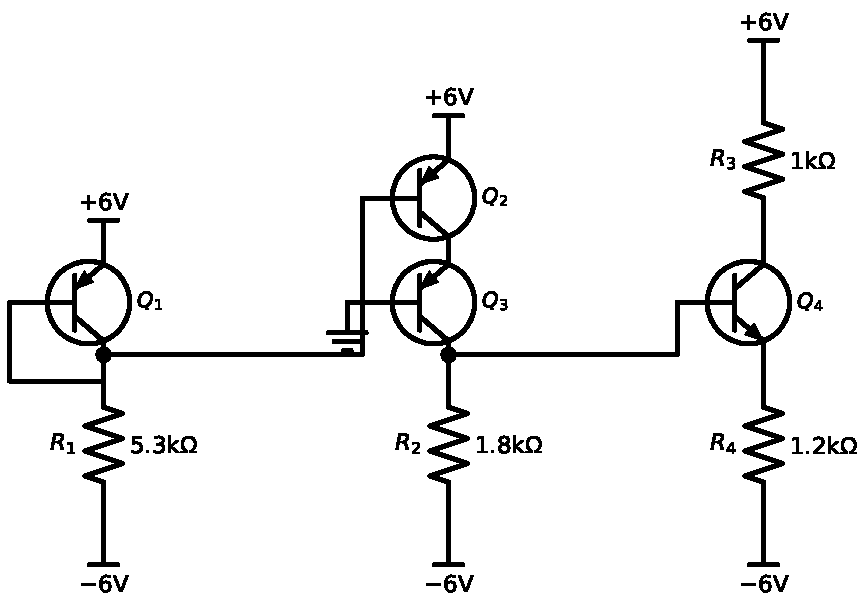
\includegraphics[width=0.9\linewidth,height=6cm,keepaspectratio]{p15_circuit}\end{center}
\solstep{1}{Assumptions}Assume every transistor is in the active region and that every base current is negligible ($I_B\approx0$, tool T1): then $|V_{BE}| = 0.7$\,V, $I_C\approx I_E$, and no current flows into any base, so a base network behaves like a plain resistor divider.
\solstep{2}{Walk through the circuit}\begin{enumerate}[leftmargin=*,itemsep=3pt]
\item $Q_{1}$ (diode-connected) is active: $V_{B1} = 6 - 0.7 = 5.3\,\mathrm{V}$.
\item $Q_{3}$ is pnp and assumed active: $V_{BE} = -0.7$\,V, so $V_{C2} = 0 + 0.7 = 0.7\,\mathrm{V}$.
\item KCL at the collector of $Q_{1}$ (base current neglected): \[I_{C1} = \frac{V_{B1} - (-6)}{R_{1}} = 2.13\,\mathrm{m}\mathrm{A}\]
\item $Q_{2}$ has the same base and emitter nodes as $Q_{1}$, hence the same $V_{BE}$ and the same current (current mirror): $I_{C2} = I_{C1} = 2.13\,\mathrm{m}\mathrm{A}$.
\item KCL at the emitter of $Q_{3}$ (base current neglected): \[I_{E3} = I_{C2} = 2.13\,\mathrm{m}\mathrm{A}, \qquad I_{C3} \approx I_{E3}\]
\item The current $I_{C3} = 2.13\,\mathrm{m}\mathrm{A}$ flows from $V_{C3}$ through $R_{2}$: $V_{C3} = (-6) + R_{2}\,(I_{C3}) = -6 + 1.8\,\mathrm{k}\times2.13\,\mathrm{m}\mathrm{A} = -2.16\,\mathrm{V}$.
\item $Q_{4}$ is npn and assumed active: $V_{BE} = 0.7$\,V, so $V_{E4} = V_{C3} - 0.7 = -2.86\,\mathrm{V}$.
\item KCL at the emitter of $Q_{4}$ (base current neglected): \[I_{E4} = \frac{V_{E4} - (-6)}{R_{4}} = 2.61\,\mathrm{m}\mathrm{A}, \qquad I_{C4} \approx I_{E4}\]
\item $Q_{4}$ draws $I_{C4} = 2.61\,\mathrm{m}\mathrm{A}$ from $V_{C4}$ through $R_{3}$: $V_{C4} = 6 - R_{3}\,(I_{C4}) = 6 - 1\,\mathrm{k}\times2.61\,\mathrm{m}\mathrm{A} = 3.39\,\mathrm{V}$.
\end{enumerate}

\solstep{3}{Verify the assumptions}\begin{itemize}[leftmargin=*,itemsep=2pt]
\item $I_{B1} = \frac{I_{C1}}{\beta} = 21.3\,\mu \mathrm{A}$ (all bases on this node: $42.6\,\mu \mathrm{A}$) $\ll$ the $2.13\,\mathrm{m}\mathrm{A}$ flowing in the base network \checkmark
\item $I_{B2} = \frac{I_{C2}}{\beta} = 21.3\,\mu \mathrm{A}$ (all bases on this node: $42.6\,\mu \mathrm{A}$) $\ll$ the $2.13\,\mathrm{m}\mathrm{A}$ flowing in the base network \checkmark
\item $I_{B4} = \frac{I_{C4}}{\beta} = 26.1\,\mu \mathrm{A}$ $\ll$ the $2.13\,\mathrm{m}\mathrm{A}$ flowing in the base network \checkmark
\item $V_{EC1} = 6 - V_{B1} = 6 - (5.3) = 0.7\,\mathrm{V}$ $\ge 0.2$\,V $\Rightarrow$ $Q_{1}$ is active \checkmark
\item $V_{EC2} = 6 - V_{C2} = 6 - (0.7) = 5.3\,\mathrm{V}$ $\ge 0.2$\,V $\Rightarrow$ $Q_{2}$ is active \checkmark
\item $V_{EC3} = V_{C2} - V_{C3} = 0.7 - (-2.162) = 2.86\,\mathrm{V}$ $\ge 0.2$\,V $\Rightarrow$ $Q_{3}$ is active \checkmark
\item $V_{CE4} = V_{C4} - V_{E4} = 3.385 - (-2.862) = 6.25\,\mathrm{V}$ $\ge 0.2$\,V $\Rightarrow$ $Q_{4}$ is active \checkmark
\end{itemize}

\solstep{4}{How good was $I_B\approx 0$?}If we keep the base currents ($I_C=\beta I_B$ with $\beta=100$) and solve the circuit exactly, the currents change only a little:\begin{center}\renewcommand{\arraystretch}{1.35}
\begin{tabular}{cccc}
\toprule
transistor & $I_C$ (with $I_B\approx0$) & $I_C$ (exact) & difference \\
\midrule
$Q_{1}$ & $2.13\,\mathrm{m}\mathrm{A}$ & $2.09\,\mathrm{m}\mathrm{A}$ & $2\%$ \\
$Q_{2}$ & $2.13\,\mathrm{m}\mathrm{A}$ & $2.09\,\mathrm{m}\mathrm{A}$ & $2\%$ \\
$Q_{3}$ & $2.13\,\mathrm{m}\mathrm{A}$ & $2.07\,\mathrm{m}\mathrm{A}$ & $3\%$ \\
$Q_{4}$ & $2.61\,\mathrm{m}\mathrm{A}$ & $2.46\,\mathrm{m}\mathrm{A}$ & $6.3\%$ \\
\bottomrule
\end{tabular}\end{center}
 The differences grow along the chain: every base current slightly shifts the collector voltage that biases the next transistor, and $\alpha = \beta/(\beta+1)$ makes each $I_C$ about 1\,\% smaller than its $I_E$. A shift is amplified when the next stage has only a small voltage across its emitter resistor. Hand analysis with $I_B\approx0$ is still the standard first pass.
\begin{ansbox}
$I_{C1} = 2.13\,\mathrm{m}\mathrm{A}$,\quad $I_{C2} = 2.13\,\mathrm{m}\mathrm{A}$,\quad $I_{C3} = 2.13\,\mathrm{m}\mathrm{A}$,\quad $I_{C4} = 2.61\,\mathrm{m}\mathrm{A}$\\[2pt] all transistors active, all base currents negligible.
\end{ansbox}

\newpage
\subsection*{Solution 4B.16 \hfill Hard}
\begin{center}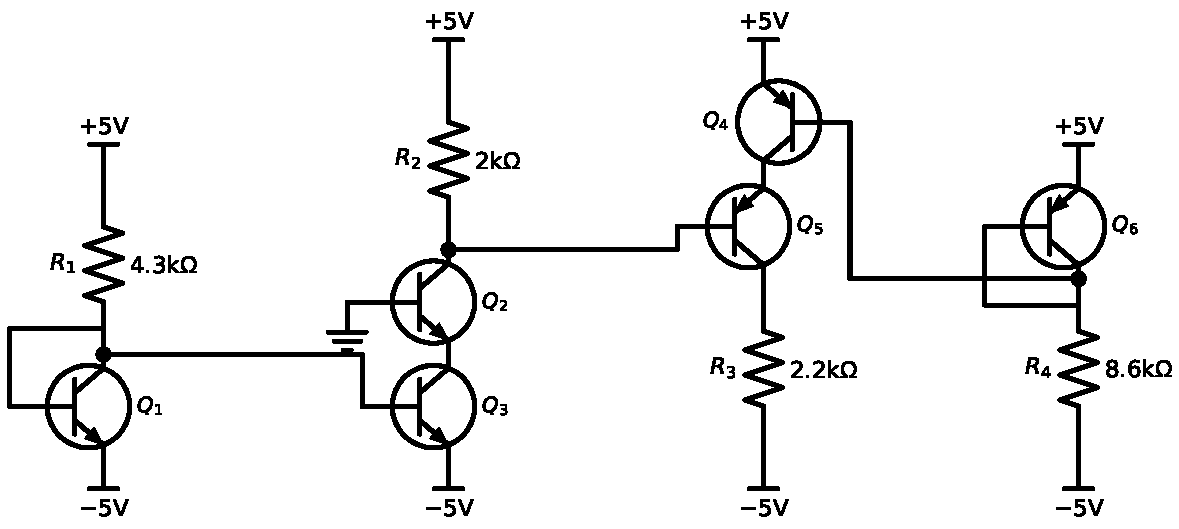
\includegraphics[width=0.9\linewidth,height=6cm,keepaspectratio]{p16_circuit}\end{center}
\solstep{1}{Assumptions}Assume every transistor is in the active region and that every base current is negligible ($I_B\approx0$, tool T1): then $|V_{BE}| = 0.7$\,V, $I_C\approx I_E$, and no current flows into any base, so a base network behaves like a plain resistor divider.
\solstep{2}{Walk through the circuit}\begin{enumerate}[leftmargin=*,itemsep=3pt]
\item $Q_{1}$ (diode-connected) is active: $V_{B1} = (-5) + 0.7 = -4.3\,\mathrm{V}$.
\item $Q_{2}$ is npn and assumed active: $V_{BE} = 0.7$\,V, so $V_{E2} = 0 - 0.7 = -0.7\,\mathrm{V}$.
\item $Q_{4}$ is active: $V_{B4} = 5 - 0.7 = 4.3\,\mathrm{V}$.
\item KCL at the collector of $Q_{1}$ (base current neglected): \[I_{C1} = \frac{5 - V_{B1}}{R_{1}} = 2.16\,\mathrm{m}\mathrm{A}\]
\item KCL at the collector of $Q_{6}$ (base current neglected): \[I_{C6} = \frac{V_{B4} - (-5)}{R_{4}} = 1.08\,\mathrm{m}\mathrm{A}\]
\item $Q_{3}$ has the same base and emitter nodes as $Q_{1}$, hence the same $V_{BE}$ and the same current (current mirror): $I_{C3} = I_{C1} = 2.16\,\mathrm{m}\mathrm{A}$.
\item $Q_{4}$ has the same base and emitter nodes as $Q_{6}$, hence the same $V_{BE}$ and the same current (current mirror): $I_{C4} = I_{C6} = 1.08\,\mathrm{m}\mathrm{A}$.
\item KCL at the emitter of $Q_{2}$ (base current neglected): \[I_{E2} = I_{C3} = 2.16\,\mathrm{m}\mathrm{A}, \qquad I_{C2} \approx I_{E2}\]
\item $Q_{2}$ draws $I_{C2} = 2.16\,\mathrm{m}\mathrm{A}$ from $V_{C2}$ through $R_{2}$: $V_{C2} = 5 - R_{2}\,(I_{C2}) = 5 - 2\,\mathrm{k}\times2.16\,\mathrm{m}\mathrm{A} = 0.674\,\mathrm{V}$.
\item $Q_{5}$ is pnp and assumed active: $V_{BE} = -0.7$\,V, so $V_{C4} = V_{C2} + 0.7 = 1.37\,\mathrm{V}$.
\item KCL at the emitter of $Q_{5}$ (base current neglected): \[I_{E5} = I_{C4} = 1.08\,\mathrm{m}\mathrm{A}, \qquad I_{C5} \approx I_{E5}\]
\item The current $I_{C5} = 1.08\,\mathrm{m}\mathrm{A}$ flows from $V_{C5}$ through $R_{3}$: $V_{C5} = (-5) + R_{3}\,(I_{C5}) = -5 + 2.2\,\mathrm{k}\times1.08\,\mathrm{m}\mathrm{A} = -2.62\,\mathrm{V}$.
\end{enumerate}

\solstep{3}{Verify the assumptions}\begin{itemize}[leftmargin=*,itemsep=2pt]
\item $I_{B1} = \frac{I_{C1}}{\beta} = 21.6\,\mu \mathrm{A}$ (all bases on this node: $43.3\,\mu \mathrm{A}$) $\ll$ the $2.16\,\mathrm{m}\mathrm{A}$ flowing in the base network \checkmark
\item $I_{B3} = \frac{I_{C3}}{\beta} = 21.6\,\mu \mathrm{A}$ (all bases on this node: $43.3\,\mu \mathrm{A}$) $\ll$ the $2.16\,\mathrm{m}\mathrm{A}$ flowing in the base network \checkmark
\item $I_{B4} = \frac{I_{C4}}{\beta} = 10.8\,\mu \mathrm{A}$ (all bases on this node: $21.6\,\mu \mathrm{A}$) $\ll$ the $1.08\,\mathrm{m}\mathrm{A}$ flowing in the base network \checkmark
\item $I_{B5} = \frac{I_{C5}}{\beta} = 10.8\,\mu \mathrm{A}$ $\ll$ the $2.16\,\mathrm{m}\mathrm{A}$ flowing in the base network \checkmark
\item $I_{B6} = \frac{I_{C6}}{\beta} = 10.8\,\mu \mathrm{A}$ (all bases on this node: $21.6\,\mu \mathrm{A}$) $\ll$ the $1.08\,\mathrm{m}\mathrm{A}$ flowing in the base network \checkmark
\item $V_{CE1} = V_{B1} - (-5) = -4.3 - (-5) = 0.7\,\mathrm{V}$ $\ge 0.2$\,V $\Rightarrow$ $Q_{1}$ is active \checkmark
\item $V_{CE2} = V_{C2} - V_{E2} = 0.6744 - (-0.7) = 1.37\,\mathrm{V}$ $\ge 0.2$\,V $\Rightarrow$ $Q_{2}$ is active \checkmark
\item $V_{CE3} = V_{E2} - (-5) = -0.7 - (-5) = 4.3\,\mathrm{V}$ $\ge 0.2$\,V $\Rightarrow$ $Q_{3}$ is active \checkmark
\item $V_{EC4} = 5 - V_{C4} = 5 - (1.374) = 3.63\,\mathrm{V}$ $\ge 0.2$\,V $\Rightarrow$ $Q_{4}$ is active \checkmark
\item $V_{EC5} = V_{C4} - V_{C5} = 1.374 - (-2.621) = 4\,\mathrm{V}$ $\ge 0.2$\,V $\Rightarrow$ $Q_{5}$ is active \checkmark
\item $V_{EC6} = 5 - V_{B4} = 5 - (4.3) = 0.7\,\mathrm{V}$ $\ge 0.2$\,V $\Rightarrow$ $Q_{6}$ is active \checkmark
\end{itemize}

\solstep{4}{How good was $I_B\approx 0$?}If we keep the base currents ($I_C=\beta I_B$ with $\beta=100$) and solve the circuit exactly, the currents change only a little:\begin{center}\renewcommand{\arraystretch}{1.35}
\begin{tabular}{cccc}
\toprule
transistor & $I_C$ (with $I_B\approx0$) & $I_C$ (exact) & difference \\
\midrule
$Q_{1}$ & $2.16\,\mathrm{m}\mathrm{A}$ & $2.12\,\mathrm{m}\mathrm{A}$ & $2\%$ \\
$Q_{2}$ & $2.16\,\mathrm{m}\mathrm{A}$ & $2.1\,\mathrm{m}\mathrm{A}$ & $3\%$ \\
$Q_{3}$ & $2.16\,\mathrm{m}\mathrm{A}$ & $2.12\,\mathrm{m}\mathrm{A}$ & $2\%$ \\
$Q_{4}$ & $1.08\,\mathrm{m}\mathrm{A}$ & $1.06\,\mathrm{m}\mathrm{A}$ & $2\%$ \\
$Q_{5}$ & $1.08\,\mathrm{m}\mathrm{A}$ & $1.05\,\mathrm{m}\mathrm{A}$ & $3\%$ \\
$Q_{6}$ & $1.08\,\mathrm{m}\mathrm{A}$ & $1.06\,\mathrm{m}\mathrm{A}$ & $2\%$ \\
\bottomrule
\end{tabular}\end{center}

\begin{ansbox}
$I_{C1} = 2.16\,\mathrm{m}\mathrm{A}$,\quad $I_{C2} = 2.16\,\mathrm{m}\mathrm{A}$,\quad $I_{C3} = 2.16\,\mathrm{m}\mathrm{A}$,\quad $I_{C4} = 1.08\,\mathrm{m}\mathrm{A}$,\quad $I_{C5} = 1.08\,\mathrm{m}\mathrm{A}$,\quad $I_{C6} = 1.08\,\mathrm{m}\mathrm{A}$\\[2pt] all transistors active, all base currents negligible.
\end{ansbox}

\newpage
\subsection*{Solution 4B.17 \hfill Hard}
\begin{center}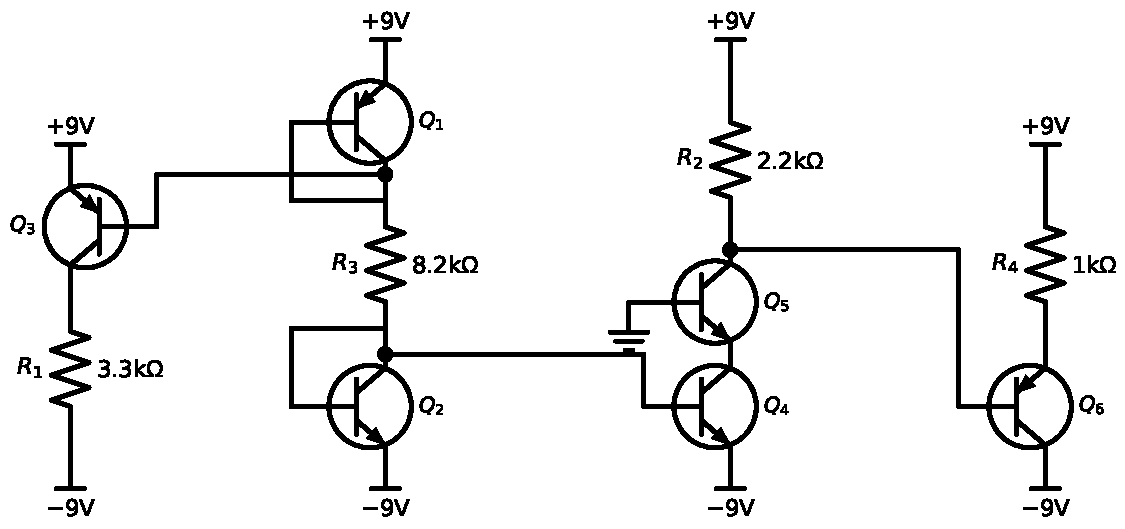
\includegraphics[width=0.9\linewidth,height=6cm,keepaspectratio]{p17_circuit}\end{center}
\solstep{1}{Assumptions}Assume every transistor is in the active region and that every base current is negligible ($I_B\approx0$, tool T1): then $|V_{BE}| = 0.7$\,V, $I_C\approx I_E$, and no current flows into any base, so a base network behaves like a plain resistor divider.
\solstep{2}{Walk through the circuit}\begin{enumerate}[leftmargin=*,itemsep=3pt]
\item $Q_{3}$ is active: $V_{B3} = 9 - 0.7 = 8.3\,\mathrm{V}$.
\item $Q_{2}$ (diode-connected) is active: $V_{B2} = (-9) + 0.7 = -8.3\,\mathrm{V}$.
\item $Q_{5}$ is npn and assumed active: $V_{BE} = 0.7$\,V, so $V_{E5} = 0 - 0.7 = -0.7\,\mathrm{V}$.
\item KCL at the collector of $Q_{2}$ (base current neglected): \[I_{C2} = \frac{V_{B3} - V_{B2}}{R_{3}} = 2.02\,\mathrm{m}\mathrm{A}\]
\item KCL at the collector of $Q_{1}$ (base current neglected): \[I_{C1} = \frac{V_{B3} - V_{B2}}{R_{3}} = 2.02\,\mathrm{m}\mathrm{A}\]
\item $Q_{3}$ has the same base and emitter nodes as $Q_{1}$, hence the same $V_{BE}$ and the same current (current mirror): $I_{C3} = I_{C1} = 2.02\,\mathrm{m}\mathrm{A}$.
\item $Q_{4}$ has the same base and emitter nodes as $Q_{2}$, hence the same $V_{BE}$ and the same current (current mirror): $I_{C4} = I_{C2} = 2.02\,\mathrm{m}\mathrm{A}$.
\item The current $I_{C3} = 2.02\,\mathrm{m}\mathrm{A}$ flows from $V_{C3}$ through $R_{1}$: $V_{C3} = (-9) + R_{1}\,(I_{C3}) = -9 + 3.3\,\mathrm{k}\times2.02\,\mathrm{m}\mathrm{A} = -2.32\,\mathrm{V}$.
\item KCL at the emitter of $Q_{5}$ (base current neglected): \[I_{E5} = I_{C4} = 2.02\,\mathrm{m}\mathrm{A}, \qquad I_{C5} \approx I_{E5}\]
\item $Q_{5}$ draws $I_{C5} = 2.02\,\mathrm{m}\mathrm{A}$ from $V_{C5}$ through $R_{2}$: $V_{C5} = 9 - R_{2}\,(I_{C5}) = 9 - 2.2\,\mathrm{k}\times2.02\,\mathrm{m}\mathrm{A} = 4.55\,\mathrm{V}$.
\item $Q_{6}$ is pnp and assumed active: $V_{BE} = -0.7$\,V, so $V_{E6} = V_{C5} + 0.7 = 5.25\,\mathrm{V}$.
\item KCL at the emitter of $Q_{6}$ (base current neglected): \[I_{E6} = \frac{9 - V_{E6}}{R_{4}} = 3.75\,\mathrm{m}\mathrm{A}, \qquad I_{C6} \approx I_{E6}\]
\end{enumerate}

\solstep{3}{Verify the assumptions}\begin{itemize}[leftmargin=*,itemsep=2pt]
\item $I_{B3} = \frac{I_{C3}}{\beta} = 20.2\,\mu \mathrm{A}$ (all bases on this node: $40.5\,\mu \mathrm{A}$) $\ll$ the $2.02\,\mathrm{m}\mathrm{A}$ flowing in the base network \checkmark
\item $I_{B1} = \frac{I_{C1}}{\beta} = 20.2\,\mu \mathrm{A}$ (all bases on this node: $40.5\,\mu \mathrm{A}$) $\ll$ the $2.02\,\mathrm{m}\mathrm{A}$ flowing in the base network \checkmark
\item $I_{B2} = \frac{I_{C2}}{\beta} = 20.2\,\mu \mathrm{A}$ (all bases on this node: $40.5\,\mu \mathrm{A}$) $\ll$ the $2.02\,\mathrm{m}\mathrm{A}$ flowing in the base network \checkmark
\item $I_{B4} = \frac{I_{C4}}{\beta} = 20.2\,\mu \mathrm{A}$ (all bases on this node: $40.5\,\mu \mathrm{A}$) $\ll$ the $2.02\,\mathrm{m}\mathrm{A}$ flowing in the base network \checkmark
\item $I_{B6} = \frac{I_{C6}}{\beta} = 37.5\,\mu \mathrm{A}$ $\ll$ the $2.02\,\mathrm{m}\mathrm{A}$ flowing in the base network \checkmark
\item $V_{EC3} = 9 - V_{C3} = 9 - (-2.32) = 11.3\,\mathrm{V}$ $\ge 0.2$\,V $\Rightarrow$ $Q_{3}$ is active \checkmark
\item $V_{EC1} = 9 - V_{B3} = 9 - (8.3) = 0.7\,\mathrm{V}$ $\ge 0.2$\,V $\Rightarrow$ $Q_{1}$ is active \checkmark
\item $V_{CE2} = V_{B2} - (-9) = -8.3 - (-9) = 0.7\,\mathrm{V}$ $\ge 0.2$\,V $\Rightarrow$ $Q_{2}$ is active \checkmark
\item $V_{CE5} = V_{C5} - V_{E5} = 4.546 - (-0.7) = 5.25\,\mathrm{V}$ $\ge 0.2$\,V $\Rightarrow$ $Q_{5}$ is active \checkmark
\item $V_{CE4} = V_{E5} - (-9) = -0.7 - (-9) = 8.3\,\mathrm{V}$ $\ge 0.2$\,V $\Rightarrow$ $Q_{4}$ is active \checkmark
\item $V_{EC6} = V_{E6} - (-9) = 5.246 - (-9) = 14.2\,\mathrm{V}$ $\ge 0.2$\,V $\Rightarrow$ $Q_{6}$ is active \checkmark
\end{itemize}

\solstep{4}{How good was $I_B\approx 0$?}If we keep the base currents ($I_C=\beta I_B$ with $\beta=100$) and solve the circuit exactly, the currents change only a little:\begin{center}\renewcommand{\arraystretch}{1.35}
\begin{tabular}{cccc}
\toprule
transistor & $I_C$ (with $I_B\approx0$) & $I_C$ (exact) & difference \\
\midrule
$Q_{3}$ & $2.02\,\mathrm{m}\mathrm{A}$ & $1.98\,\mathrm{m}\mathrm{A}$ & $2\%$ \\
$Q_{1}$ & $2.02\,\mathrm{m}\mathrm{A}$ & $1.98\,\mathrm{m}\mathrm{A}$ & $2\%$ \\
$Q_{2}$ & $2.02\,\mathrm{m}\mathrm{A}$ & $1.98\,\mathrm{m}\mathrm{A}$ & $2\%$ \\
$Q_{5}$ & $2.02\,\mathrm{m}\mathrm{A}$ & $1.97\,\mathrm{m}\mathrm{A}$ & $3\%$ \\
$Q_{4}$ & $2.02\,\mathrm{m}\mathrm{A}$ & $1.98\,\mathrm{m}\mathrm{A}$ & $2\%$ \\
$Q_{6}$ & $3.75\,\mathrm{m}\mathrm{A}$ & $3.51\,\mathrm{m}\mathrm{A}$ & $6.9\%$ \\
\bottomrule
\end{tabular}\end{center}
 The differences grow along the chain: every base current slightly shifts the collector voltage that biases the next transistor, and $\alpha = \beta/(\beta+1)$ makes each $I_C$ about 1\,\% smaller than its $I_E$. A shift is amplified when the next stage has only a small voltage across its emitter resistor. Hand analysis with $I_B\approx0$ is still the standard first pass.
\begin{ansbox}
$I_{C3} = 2.02\,\mathrm{m}\mathrm{A}$,\quad $I_{C1} = 2.02\,\mathrm{m}\mathrm{A}$,\quad $I_{C2} = 2.02\,\mathrm{m}\mathrm{A}$,\quad $I_{C5} = 2.02\,\mathrm{m}\mathrm{A}$,\quad $I_{C4} = 2.02\,\mathrm{m}\mathrm{A}$,\quad $I_{C6} = 3.75\,\mathrm{m}\mathrm{A}$\\[2pt] all transistors active, all base currents negligible.
\end{ansbox}

\newpage
\subsection*{Solution 4B.18 \hfill Hard}
\begin{center}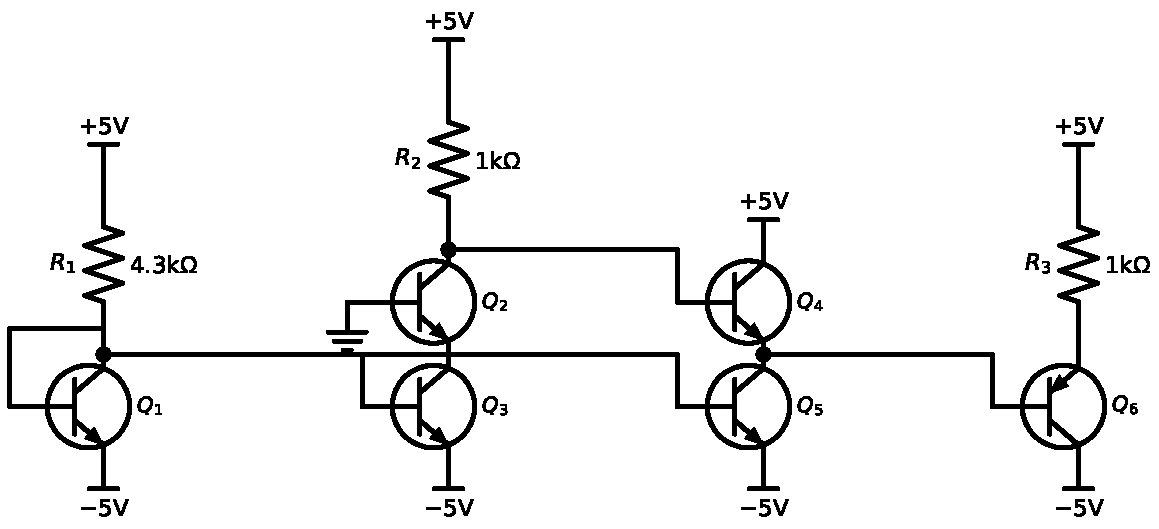
\includegraphics[width=0.9\linewidth,height=6cm,keepaspectratio]{p18_circuit}\end{center}
\solstep{1}{Assumptions}Assume every transistor is in the active region and that every base current is negligible ($I_B\approx0$, tool T1): then $|V_{BE}| = 0.7$\,V, $I_C\approx I_E$, and no current flows into any base, so a base network behaves like a plain resistor divider.
\solstep{2}{Walk through the circuit}\begin{enumerate}[leftmargin=*,itemsep=3pt]
\item $Q_{1}$ (diode-connected) is active: $V_{B1} = (-5) + 0.7 = -4.3\,\mathrm{V}$.
\item $Q_{2}$ is npn and assumed active: $V_{BE} = 0.7$\,V, so $V_{E2} = 0 - 0.7 = -0.7\,\mathrm{V}$.
\item KCL at the collector of $Q_{1}$ (base current neglected): \[I_{C1} = \frac{5 - V_{B1}}{R_{1}} = 2.16\,\mathrm{m}\mathrm{A}\]
\item $Q_{3}$ has the same base and emitter nodes as $Q_{1}$, hence the same $V_{BE}$ and the same current (current mirror): $I_{C3} = I_{C1} = 2.16\,\mathrm{m}\mathrm{A}$.
\item $Q_{5}$ has the same base and emitter nodes as $Q_{1}$, hence the same $V_{BE}$ and the same current (current mirror): $I_{C5} = I_{C1} = 2.16\,\mathrm{m}\mathrm{A}$.
\item KCL at the emitter of $Q_{2}$ (base current neglected): \[I_{E2} = I_{C3} = 2.16\,\mathrm{m}\mathrm{A}, \qquad I_{C2} \approx I_{E2}\]
\item $Q_{2}$ draws $I_{C2} = 2.16\,\mathrm{m}\mathrm{A}$ from $V_{C2}$ through $R_{2}$: $V_{C2} = 5 - R_{2}\,(I_{C2}) = 5 - 1\,\mathrm{k}\times2.16\,\mathrm{m}\mathrm{A} = 2.84\,\mathrm{V}$.
\item $Q_{4}$ is npn and assumed active: $V_{BE} = 0.7$\,V, so $V_{E4} = V_{C2} - 0.7 = 2.14\,\mathrm{V}$.
\item $Q_{6}$ is pnp and assumed active: $V_{BE} = -0.7$\,V, so $V_{E6} = V_{E4} + 0.7 = 2.84\,\mathrm{V}$.
\item KCL at the emitter of $Q_{4}$ (base current neglected): \[I_{E4} = I_{C5} = 2.16\,\mathrm{m}\mathrm{A}, \qquad I_{C4} \approx I_{E4}\]
\item KCL at the emitter of $Q_{6}$ (base current neglected): \[I_{E6} = \frac{5 - V_{E6}}{R_{3}} = 2.16\,\mathrm{m}\mathrm{A}, \qquad I_{C6} \approx I_{E6}\]
\end{enumerate}

\solstep{3}{Verify the assumptions}\begin{itemize}[leftmargin=*,itemsep=2pt]
\item $I_{B1} = \frac{I_{C1}}{\beta} = 21.6\,\mu \mathrm{A}$ (all bases on this node: $64.9\,\mu \mathrm{A}$) $\ll$ the $2.16\,\mathrm{m}\mathrm{A}$ flowing in the base network \checkmark
\item $I_{B3} = \frac{I_{C3}}{\beta} = 21.6\,\mu \mathrm{A}$ (all bases on this node: $64.9\,\mu \mathrm{A}$) $\ll$ the $2.16\,\mathrm{m}\mathrm{A}$ flowing in the base network \checkmark
\item $I_{B4} = \frac{I_{C4}}{\beta} = 21.6\,\mu \mathrm{A}$ $\ll$ the $2.16\,\mathrm{m}\mathrm{A}$ flowing in the base network \checkmark
\item $I_{B5} = \frac{I_{C5}}{\beta} = 21.6\,\mu \mathrm{A}$ (all bases on this node: $64.9\,\mu \mathrm{A}$) $\ll$ the $2.16\,\mathrm{m}\mathrm{A}$ flowing in the base network \checkmark
\item $V_{CE1} = V_{B1} - (-5) = -4.3 - (-5) = 0.7\,\mathrm{V}$ $\ge 0.2$\,V $\Rightarrow$ $Q_{1}$ is active \checkmark
\item $V_{CE2} = V_{C2} - V_{E2} = 2.837 - (-0.7) = 3.54\,\mathrm{V}$ $\ge 0.2$\,V $\Rightarrow$ $Q_{2}$ is active \checkmark
\item $V_{CE3} = V_{E2} - (-5) = -0.7 - (-5) = 4.3\,\mathrm{V}$ $\ge 0.2$\,V $\Rightarrow$ $Q_{3}$ is active \checkmark
\item $V_{CE4} = 5 - V_{E4} = 5 - (2.137) = 2.86\,\mathrm{V}$ $\ge 0.2$\,V $\Rightarrow$ $Q_{4}$ is active \checkmark
\item $V_{CE5} = V_{E4} - (-5) = 2.137 - (-5) = 7.14\,\mathrm{V}$ $\ge 0.2$\,V $\Rightarrow$ $Q_{5}$ is active \checkmark
\item $V_{EC6} = V_{E6} - (-5) = 2.837 - (-5) = 7.84\,\mathrm{V}$ $\ge 0.2$\,V $\Rightarrow$ $Q_{6}$ is active \checkmark
\end{itemize}

\solstep{4}{How good was $I_B\approx 0$?}If we keep the base currents ($I_C=\beta I_B$ with $\beta=100$) and solve the circuit exactly, the currents change only a little:\begin{center}\renewcommand{\arraystretch}{1.35}
\begin{tabular}{cccc}
\toprule
transistor & $I_C$ (with $I_B\approx0$) & $I_C$ (exact) & difference \\
\midrule
$Q_{1}$ & $2.16\,\mathrm{m}\mathrm{A}$ & $2.1\,\mathrm{m}\mathrm{A}$ & $3\%$ \\
$Q_{2}$ & $2.16\,\mathrm{m}\mathrm{A}$ & $2.08\,\mathrm{m}\mathrm{A}$ & $4\%$ \\
$Q_{3}$ & $2.16\,\mathrm{m}\mathrm{A}$ & $2.1\,\mathrm{m}\mathrm{A}$ & $3\%$ \\
$Q_{4}$ & $2.16\,\mathrm{m}\mathrm{A}$ & $2.06\,\mathrm{m}\mathrm{A}$ & $5.1\%$ \\
$Q_{5}$ & $2.16\,\mathrm{m}\mathrm{A}$ & $2.1\,\mathrm{m}\mathrm{A}$ & $3\%$ \\
$Q_{6}$ & $2.16\,\mathrm{m}\mathrm{A}$ & $2.08\,\mathrm{m}\mathrm{A}$ & $4\%$ \\
\bottomrule
\end{tabular}\end{center}

\begin{ansbox}
$I_{C1} = 2.16\,\mathrm{m}\mathrm{A}$,\quad $I_{C2} = 2.16\,\mathrm{m}\mathrm{A}$,\quad $I_{C3} = 2.16\,\mathrm{m}\mathrm{A}$,\quad $I_{C4} = 2.16\,\mathrm{m}\mathrm{A}$,\quad $I_{C5} = 2.16\,\mathrm{m}\mathrm{A}$,\quad $I_{C6} = 2.16\,\mathrm{m}\mathrm{A}$\\[2pt] all transistors active, all base currents negligible.
\end{ansbox}

\end{document}
